\documentclass[twoside]{book}

% Packages required by doxygen
\usepackage{fixltx2e}
\usepackage{calc}
\usepackage{doxygen}
\usepackage[export]{adjustbox} % also loads graphicx
\usepackage{graphicx}
\usepackage[utf8]{inputenc}
\usepackage{makeidx}
\usepackage{multicol}
\usepackage{multirow}
\PassOptionsToPackage{warn}{textcomp}
\usepackage{textcomp}
\usepackage[nointegrals]{wasysym}
\usepackage[table]{xcolor}

% Font selection
\usepackage[T1]{fontenc}
\usepackage[scaled=.90]{helvet}
\usepackage{courier}
\usepackage{amssymb}
\usepackage{sectsty}
\renewcommand{\familydefault}{\sfdefault}
\allsectionsfont{%
  \fontseries{bc}\selectfont%
  \color{darkgray}%
}
\renewcommand{\DoxyLabelFont}{%
  \fontseries{bc}\selectfont%
  \color{darkgray}%
}
\newcommand{\+}{\discretionary{\mbox{\scriptsize$\hookleftarrow$}}{}{}}

% Page & text layout
\usepackage{geometry}
\geometry{%
  a4paper,%
  top=2.5cm,%
  bottom=2.5cm,%
  left=2.5cm,%
  right=2.5cm%
}
\tolerance=750
\hfuzz=15pt
\hbadness=750
\setlength{\emergencystretch}{15pt}
\setlength{\parindent}{0cm}
\setlength{\parskip}{3ex plus 2ex minus 2ex}
\makeatletter
\renewcommand{\paragraph}{%
  \@startsection{paragraph}{4}{0ex}{-1.0ex}{1.0ex}{%
    \normalfont\normalsize\bfseries\SS@parafont%
  }%
}
\renewcommand{\subparagraph}{%
  \@startsection{subparagraph}{5}{0ex}{-1.0ex}{1.0ex}{%
    \normalfont\normalsize\bfseries\SS@subparafont%
  }%
}
\makeatother

% Headers & footers
\usepackage{fancyhdr}
\pagestyle{fancyplain}
\fancyhead[LE]{\fancyplain{}{\bfseries\thepage}}
\fancyhead[CE]{\fancyplain{}{}}
\fancyhead[RE]{\fancyplain{}{\bfseries\leftmark}}
\fancyhead[LO]{\fancyplain{}{\bfseries\rightmark}}
\fancyhead[CO]{\fancyplain{}{}}
\fancyhead[RO]{\fancyplain{}{\bfseries\thepage}}
\fancyfoot[LE]{\fancyplain{}{}}
\fancyfoot[CE]{\fancyplain{}{}}
\fancyfoot[RE]{\fancyplain{}{\bfseries\scriptsize Generated by Doxygen }}
\fancyfoot[LO]{\fancyplain{}{\bfseries\scriptsize Generated by Doxygen }}
\fancyfoot[CO]{\fancyplain{}{}}
\fancyfoot[RO]{\fancyplain{}{}}
\renewcommand{\footrulewidth}{0.4pt}
\renewcommand{\chaptermark}[1]{%
  \markboth{#1}{}%
}
\renewcommand{\sectionmark}[1]{%
  \markright{\thesection\ #1}%
}

% Indices & bibliography
\usepackage{natbib}
\usepackage[titles]{tocloft}
\setcounter{tocdepth}{3}
\setcounter{secnumdepth}{5}
\makeindex

% Hyperlinks (required, but should be loaded last)
\usepackage{ifpdf}
\ifpdf
  \usepackage[pdftex,pagebackref=true]{hyperref}
\else
  \usepackage[ps2pdf,pagebackref=true]{hyperref}
\fi
\hypersetup{%
  colorlinks=true,%
  linkcolor=blue,%
  citecolor=blue,%
  unicode%
}

% Custom commands
\newcommand{\clearemptydoublepage}{%
  \newpage{\pagestyle{empty}\cleardoublepage}%
}

\usepackage{caption}
\captionsetup{labelsep=space,justification=centering,font={bf},singlelinecheck=off,skip=4pt,position=top}

%===== C O N T E N T S =====

\begin{document}

% Titlepage & ToC
\hypersetup{pageanchor=false,
             bookmarksnumbered=true,
             pdfencoding=unicode
            }
\pagenumbering{roman}
\begin{titlepage}
\vspace*{7cm}
\begin{center}%
{\Large Heisprosjekt }\\
\vspace*{1cm}
{\large Generated by Doxygen 1.8.11}\\
\end{center}
\end{titlepage}
\clearemptydoublepage
\tableofcontents
\clearemptydoublepage
\pagenumbering{arabic}
\hypersetup{pageanchor=true}

%--- Begin generated contents ---
\chapter{File Index}
\section{File List}
Here is a list of all documented files with brief descriptions\+:\begin{DoxyCompactList}
\item\contentsline{section}{source/{\bfseries channels.\+h} }{\pageref{channels_8h}}{}
\item\contentsline{section}{source/{\bfseries elev.\+c} }{\pageref{elev_8c}}{}
\item\contentsline{section}{source/\hyperlink{elev_8h}{elev.\+h} \\*A library containing functions regarding the elev (elevator) module }{\pageref{elev_8h}}{}
\item\contentsline{section}{source/{\bfseries F\+S\+M.\+c} }{\pageref{FSM_8c}}{}
\item\contentsline{section}{source/\hyperlink{FSM_8h}{F\+S\+M.\+h} \\*A library containing functions regarding the F\+SM (Finite-\/state machine) module }{\pageref{FSM_8h}}{}
\item\contentsline{section}{source/{\bfseries io.\+c} }{\pageref{io_8c}}{}
\item\contentsline{section}{source/\hyperlink{io_8h}{io.\+h} \\*A library containing functions regarding the io (in/out) module }{\pageref{io_8h}}{}
\item\contentsline{section}{source/{\bfseries lights.\+c} }{\pageref{lights_8c}}{}
\item\contentsline{section}{source/\hyperlink{lights_8h}{lights.\+h} \\*A library containing the functions regarding the lights module }{\pageref{lights_8h}}{}
\item\contentsline{section}{source/\hyperlink{main_8c}{main.\+c} \\*File for the main function of the program }{\pageref{main_8c}}{}
\item\contentsline{section}{source/{\bfseries queue.\+c} }{\pageref{queue_8c}}{}
\item\contentsline{section}{source/\hyperlink{queue_8h}{queue.\+h} \\*A library containing functions regarding the queue module }{\pageref{queue_8h}}{}
\item\contentsline{section}{source/{\bfseries timer.\+c} }{\pageref{timer_8c}}{}
\item\contentsline{section}{source/\hyperlink{timer_8h}{timer.\+h} \\*A library containing functions regarding the timer module }{\pageref{timer_8h}}{}
\end{DoxyCompactList}

\chapter{File Documentation}
\hypertarget{channels_8h}{}\section{source/channels.h File Reference}
\label{channels_8h}\index{source/channels.\+h@{source/channels.\+h}}


Channel definition for elevator using Lib\+Comedi.  


This graph shows which files directly or indirectly include this file\+:
\nopagebreak
\begin{figure}[H]
\begin{center}
\leavevmode
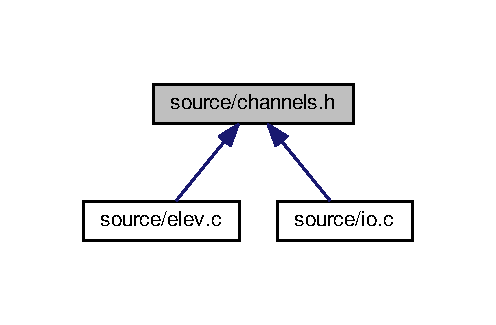
\includegraphics[width=238pt]{channels_8h__dep__incl}
\end{center}
\end{figure}
\subsection*{Macros}
\begin{DoxyCompactItemize}
\item 
\#define {\bfseries P\+O\+R\+T4}~3\hypertarget{channels_8h_ad5a54f368997d8ae4f84a1e2fad533f4}{}\label{channels_8h_ad5a54f368997d8ae4f84a1e2fad533f4}

\item 
\#define {\bfseries O\+B\+S\+T\+R\+U\+C\+T\+I\+ON}~(0x300+23)\hypertarget{channels_8h_a2409f02d98d288f64712887bd13b853e}{}\label{channels_8h_a2409f02d98d288f64712887bd13b853e}

\item 
\#define {\bfseries S\+T\+OP}~(0x300+22)\hypertarget{channels_8h_ae19b6bb2940d2fbe0a79852b070eeafd}{}\label{channels_8h_ae19b6bb2940d2fbe0a79852b070eeafd}

\item 
\#define {\bfseries B\+U\+T\+T\+O\+N\+\_\+\+C\+O\+M\+M\+A\+N\+D1}~(0x300+21)\hypertarget{channels_8h_a1a22e01173ae543c7350d23af9099083}{}\label{channels_8h_a1a22e01173ae543c7350d23af9099083}

\item 
\#define {\bfseries B\+U\+T\+T\+O\+N\+\_\+\+C\+O\+M\+M\+A\+N\+D2}~(0x300+20)\hypertarget{channels_8h_a8f3d02fddfb1ecd5227eca135f19ebd6}{}\label{channels_8h_a8f3d02fddfb1ecd5227eca135f19ebd6}

\item 
\#define {\bfseries B\+U\+T\+T\+O\+N\+\_\+\+C\+O\+M\+M\+A\+N\+D3}~(0x300+19)\hypertarget{channels_8h_a82aab21b1b50d554effcf8b26576b388}{}\label{channels_8h_a82aab21b1b50d554effcf8b26576b388}

\item 
\#define {\bfseries B\+U\+T\+T\+O\+N\+\_\+\+C\+O\+M\+M\+A\+N\+D4}~(0x300+18)\hypertarget{channels_8h_add9ae7df96dfd4ad569d3b703023187d}{}\label{channels_8h_add9ae7df96dfd4ad569d3b703023187d}

\item 
\#define {\bfseries B\+U\+T\+T\+O\+N\+\_\+\+U\+P1}~(0x300+17)\hypertarget{channels_8h_a7236f6ea90139248afabe014632c3cec}{}\label{channels_8h_a7236f6ea90139248afabe014632c3cec}

\item 
\#define {\bfseries B\+U\+T\+T\+O\+N\+\_\+\+U\+P2}~(0x300+16)\hypertarget{channels_8h_a3a95d31cf2002937c921bbd85590bc7a}{}\label{channels_8h_a3a95d31cf2002937c921bbd85590bc7a}

\item 
\#define {\bfseries P\+O\+R\+T1}~2\hypertarget{channels_8h_a83b698b796fa8d1625536439f28ea575}{}\label{channels_8h_a83b698b796fa8d1625536439f28ea575}

\item 
\#define {\bfseries B\+U\+T\+T\+O\+N\+\_\+\+D\+O\+W\+N2}~(0x200+0)\hypertarget{channels_8h_a63a7b9d9d7c23325d4171292d596fa11}{}\label{channels_8h_a63a7b9d9d7c23325d4171292d596fa11}

\item 
\#define {\bfseries B\+U\+T\+T\+O\+N\+\_\+\+U\+P3}~(0x200+1)\hypertarget{channels_8h_aa6b5917715e012cf21e3a89fb7c93e2d}{}\label{channels_8h_aa6b5917715e012cf21e3a89fb7c93e2d}

\item 
\#define {\bfseries B\+U\+T\+T\+O\+N\+\_\+\+D\+O\+W\+N3}~(0x200+2)\hypertarget{channels_8h_ab423174da71ed0d6b083cd8d71f54617}{}\label{channels_8h_ab423174da71ed0d6b083cd8d71f54617}

\item 
\#define {\bfseries B\+U\+T\+T\+O\+N\+\_\+\+D\+O\+W\+N4}~(0x200+3)\hypertarget{channels_8h_a7e1266fcb6843826718edec0222b1e49}{}\label{channels_8h_a7e1266fcb6843826718edec0222b1e49}

\item 
\#define {\bfseries S\+E\+N\+S\+O\+R\+\_\+\+F\+L\+O\+O\+R1}~(0x200+4)\hypertarget{channels_8h_a5ae95fe4e1273653467895d5e7c39377}{}\label{channels_8h_a5ae95fe4e1273653467895d5e7c39377}

\item 
\#define {\bfseries S\+E\+N\+S\+O\+R\+\_\+\+F\+L\+O\+O\+R2}~(0x200+5)\hypertarget{channels_8h_ab9e1c393bf2c51d65ed0a132af8321d3}{}\label{channels_8h_ab9e1c393bf2c51d65ed0a132af8321d3}

\item 
\#define {\bfseries S\+E\+N\+S\+O\+R\+\_\+\+F\+L\+O\+O\+R3}~(0x200+6)\hypertarget{channels_8h_a65904322d022513386fea3bcb9a8b524}{}\label{channels_8h_a65904322d022513386fea3bcb9a8b524}

\item 
\#define {\bfseries S\+E\+N\+S\+O\+R\+\_\+\+F\+L\+O\+O\+R4}~(0x200+7)\hypertarget{channels_8h_a6a8d30abdce8780479ac7f0677200074}{}\label{channels_8h_a6a8d30abdce8780479ac7f0677200074}

\item 
\#define {\bfseries P\+O\+R\+T3}~3\hypertarget{channels_8h_ad906b7f6a811f1f02b5eb04cbe1bc89b}{}\label{channels_8h_ad906b7f6a811f1f02b5eb04cbe1bc89b}

\item 
\#define {\bfseries M\+O\+T\+O\+R\+D\+IR}~(0x300+15)\hypertarget{channels_8h_aaa316c7fc13ca7b9b4229af3f9832a7d}{}\label{channels_8h_aaa316c7fc13ca7b9b4229af3f9832a7d}

\item 
\#define {\bfseries L\+I\+G\+H\+T\+\_\+\+S\+T\+OP}~(0x300+14)\hypertarget{channels_8h_a7845eb8e4ab5e0a49739663d69ff9001}{}\label{channels_8h_a7845eb8e4ab5e0a49739663d69ff9001}

\item 
\#define {\bfseries L\+I\+G\+H\+T\+\_\+\+C\+O\+M\+M\+A\+N\+D1}~(0x300+13)\hypertarget{channels_8h_a61e8bfbed9e1d63bbbce251b10b69d9b}{}\label{channels_8h_a61e8bfbed9e1d63bbbce251b10b69d9b}

\item 
\#define {\bfseries L\+I\+G\+H\+T\+\_\+\+C\+O\+M\+M\+A\+N\+D2}~(0x300+12)\hypertarget{channels_8h_a05423733c25f39ca059f5bfae9e3fb33}{}\label{channels_8h_a05423733c25f39ca059f5bfae9e3fb33}

\item 
\#define {\bfseries L\+I\+G\+H\+T\+\_\+\+C\+O\+M\+M\+A\+N\+D3}~(0x300+11)\hypertarget{channels_8h_aec8c2b567fd77cff4163ebab81b6abd1}{}\label{channels_8h_aec8c2b567fd77cff4163ebab81b6abd1}

\item 
\#define {\bfseries L\+I\+G\+H\+T\+\_\+\+C\+O\+M\+M\+A\+N\+D4}~(0x300+10)\hypertarget{channels_8h_ad2ffefe386fcbad6a538f84c7fe191f3}{}\label{channels_8h_ad2ffefe386fcbad6a538f84c7fe191f3}

\item 
\#define {\bfseries L\+I\+G\+H\+T\+\_\+\+U\+P1}~(0x300+9)\hypertarget{channels_8h_aec0494e52bb28dfa15a8035c3359bd0f}{}\label{channels_8h_aec0494e52bb28dfa15a8035c3359bd0f}

\item 
\#define {\bfseries L\+I\+G\+H\+T\+\_\+\+U\+P2}~(0x300+8)\hypertarget{channels_8h_ab4f192467448356764080a8102eb32f1}{}\label{channels_8h_ab4f192467448356764080a8102eb32f1}

\item 
\#define {\bfseries P\+O\+R\+T2}~3\hypertarget{channels_8h_acb270e4aec8a0ab123e6c24a5810150b}{}\label{channels_8h_acb270e4aec8a0ab123e6c24a5810150b}

\item 
\#define {\bfseries L\+I\+G\+H\+T\+\_\+\+D\+O\+W\+N2}~(0x300+7)\hypertarget{channels_8h_a919d92344f7934414150b99fe94d1ace}{}\label{channels_8h_a919d92344f7934414150b99fe94d1ace}

\item 
\#define {\bfseries L\+I\+G\+H\+T\+\_\+\+U\+P3}~(0x300+6)\hypertarget{channels_8h_a2fd78cafe153eb500f5f6731f6a2d7c7}{}\label{channels_8h_a2fd78cafe153eb500f5f6731f6a2d7c7}

\item 
\#define {\bfseries L\+I\+G\+H\+T\+\_\+\+D\+O\+W\+N3}~(0x300+5)\hypertarget{channels_8h_adc5182903fbf37402ed9a2b65af65a40}{}\label{channels_8h_adc5182903fbf37402ed9a2b65af65a40}

\item 
\#define {\bfseries L\+I\+G\+H\+T\+\_\+\+D\+O\+W\+N4}~(0x300+4)\hypertarget{channels_8h_a1745b9fd720072a9ff8f58c75ca9512c}{}\label{channels_8h_a1745b9fd720072a9ff8f58c75ca9512c}

\item 
\#define {\bfseries L\+I\+G\+H\+T\+\_\+\+D\+O\+O\+R\+\_\+\+O\+P\+EN}~(0x300+3)\hypertarget{channels_8h_ab3e81b38bff9c0c8dd9dea97f3c42073}{}\label{channels_8h_ab3e81b38bff9c0c8dd9dea97f3c42073}

\item 
\#define {\bfseries L\+I\+G\+H\+T\+\_\+\+F\+L\+O\+O\+R\+\_\+\+I\+N\+D2}~(0x300+1)\hypertarget{channels_8h_a99e7a2989cfe5f085c49c31d033baae2}{}\label{channels_8h_a99e7a2989cfe5f085c49c31d033baae2}

\item 
\#define {\bfseries L\+I\+G\+H\+T\+\_\+\+F\+L\+O\+O\+R\+\_\+\+I\+N\+D1}~(0x300+0)\hypertarget{channels_8h_a1b686be38adf6a919cceca00890df7c8}{}\label{channels_8h_a1b686be38adf6a919cceca00890df7c8}

\item 
\#define {\bfseries P\+O\+R\+T0}~1\hypertarget{channels_8h_af41b34488a518db05b413d3a370f871f}{}\label{channels_8h_af41b34488a518db05b413d3a370f871f}

\item 
\#define {\bfseries M\+O\+T\+OR}~(0x100+0)\hypertarget{channels_8h_ae8d3b23b31729f61bc738fbd9a9a24e0}{}\label{channels_8h_ae8d3b23b31729f61bc738fbd9a9a24e0}

\item 
\#define {\bfseries B\+U\+T\+T\+O\+N\+\_\+\+D\+O\+W\+N1}~-\/1\hypertarget{channels_8h_a8bcc98057f83b3b335fa3d9865410d42}{}\label{channels_8h_a8bcc98057f83b3b335fa3d9865410d42}

\item 
\#define {\bfseries B\+U\+T\+T\+O\+N\+\_\+\+U\+P4}~-\/1\hypertarget{channels_8h_a02cc4cce547c81453cf7b5e55dd24986}{}\label{channels_8h_a02cc4cce547c81453cf7b5e55dd24986}

\item 
\#define {\bfseries L\+I\+G\+H\+T\+\_\+\+D\+O\+W\+N1}~-\/1\hypertarget{channels_8h_ad63056bd0003fdef7bdf927bf2ff1118}{}\label{channels_8h_ad63056bd0003fdef7bdf927bf2ff1118}

\item 
\#define {\bfseries L\+I\+G\+H\+T\+\_\+\+U\+P4}~-\/1\hypertarget{channels_8h_ab4e1e3be316a23e33d3080931737eb60}{}\label{channels_8h_ab4e1e3be316a23e33d3080931737eb60}

\end{DoxyCompactItemize}


\subsection{Detailed Description}
Channel definition for elevator using Lib\+Comedi. 


\hypertarget{elev_8c}{}\section{source/elev.c File Reference}
\label{elev_8c}\index{source/elev.\+c@{source/elev.\+c}}


Implementation file regarding the elev (elevator) module.  


{\ttfamily \#include \char`\"{}channels.\+h\char`\"{}}\\*
{\ttfamily \#include \char`\"{}elev.\+h\char`\"{}}\\*
{\ttfamily \#include \char`\"{}io.\+h\char`\"{}}\\*
{\ttfamily \#include $<$assert.\+h$>$}\\*
{\ttfamily \#include $<$stdlib.\+h$>$}\\*
Include dependency graph for elev.\+c\+:
\nopagebreak
\begin{figure}[H]
\begin{center}
\leavevmode
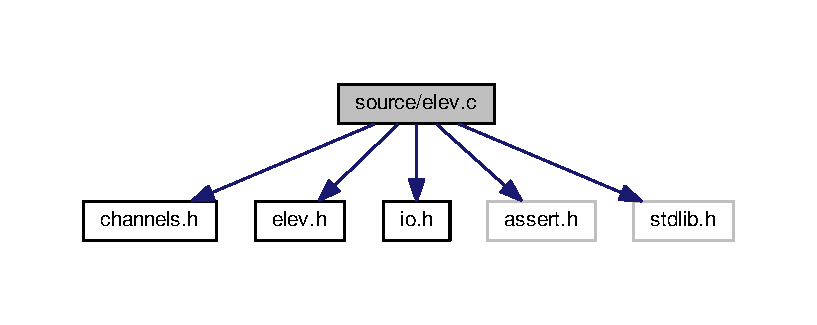
\includegraphics[width=350pt]{elev_8c__incl}
\end{center}
\end{figure}
\subsection*{Macros}
\begin{DoxyCompactItemize}
\item 
\#define {\bfseries N\+\_\+\+B\+U\+T\+T\+O\+NS}~3\hypertarget{elev_8c_a271dda243b0f5bd7d2053d258eb71962}{}\label{elev_8c_a271dda243b0f5bd7d2053d258eb71962}

\end{DoxyCompactItemize}
\subsection*{Functions}
\begin{DoxyCompactItemize}
\item 
int \hyperlink{elev_8c_a949b0e1f7c0f03ea6f92008c378e4573}{elev\+\_\+init} (void)
\item 
void \hyperlink{elev_8c_ac7dccb879f6e812e9d245174a0214536}{elev\+\_\+set\+\_\+motor\+\_\+direction} (\hyperlink{elev_8h_a2256dfd58fecce253106f83fd2ed607f}{elev\+\_\+motor\+\_\+direction\+\_\+t} dirn)
\item 
void \hyperlink{elev_8c_a6ce9a34b8677b483b0d8f9dc47b42c40}{elev\+\_\+set\+\_\+door\+\_\+open\+\_\+lamp} (int value)
\item 
int \hyperlink{elev_8c_acd97a0fbc9013dc954923e25e90be9df}{elev\+\_\+get\+\_\+obstruction\+\_\+signal} (void)
\item 
int \hyperlink{elev_8c_ab702d0ff2d7d03172b7ae3829ba13028}{elev\+\_\+get\+\_\+stop\+\_\+signal} (void)
\item 
void \hyperlink{elev_8c_a85de2a6536b4dd0c83bac19923500740}{elev\+\_\+set\+\_\+stop\+\_\+lamp} (int value)
\item 
int \hyperlink{elev_8c_a97d30b7e2538acf5647515638070fdc5}{elev\+\_\+get\+\_\+floor\+\_\+sensor\+\_\+signal} (void)
\item 
void \hyperlink{elev_8c_a6af53dd3ebae3a5791ba345eac84d4be}{elev\+\_\+set\+\_\+floor\+\_\+indicator} (int floor)
\item 
int \hyperlink{elev_8c_a2350a1635233760719700552a6cb0763}{elev\+\_\+get\+\_\+button\+\_\+signal} (\hyperlink{elev_8h_af61c4136fb437a2c49037e5a57c9abda}{elev\+\_\+button\+\_\+type\+\_\+t} button, int floor)
\item 
void \hyperlink{elev_8c_a9e81321c63d80ddf1699bc91593cd9d4}{elev\+\_\+set\+\_\+button\+\_\+lamp} (\hyperlink{elev_8h_af61c4136fb437a2c49037e5a57c9abda}{elev\+\_\+button\+\_\+type\+\_\+t} button, int floor, int value)
\end{DoxyCompactItemize}


\subsection{Detailed Description}
Implementation file regarding the elev (elevator) module. 



\subsection{Function Documentation}
\index{elev.\+c@{elev.\+c}!elev\+\_\+get\+\_\+button\+\_\+signal@{elev\+\_\+get\+\_\+button\+\_\+signal}}
\index{elev\+\_\+get\+\_\+button\+\_\+signal@{elev\+\_\+get\+\_\+button\+\_\+signal}!elev.\+c@{elev.\+c}}
\subsubsection[{\texorpdfstring{elev\+\_\+get\+\_\+button\+\_\+signal(elev\+\_\+button\+\_\+type\+\_\+t button, int floor)}{elev_get_button_signal(elev_button_type_t button, int floor)}}]{\setlength{\rightskip}{0pt plus 5cm}int elev\+\_\+get\+\_\+button\+\_\+signal (
\begin{DoxyParamCaption}
\item[{{\bf elev\+\_\+button\+\_\+type\+\_\+t}}]{button, }
\item[{int}]{floor}
\end{DoxyParamCaption}
)}\hypertarget{elev_8c_a2350a1635233760719700552a6cb0763}{}\label{elev_8c_a2350a1635233760719700552a6cb0763}
Gets a button signal. 
\begin{DoxyParams}{Parameters}
{\em button} & Which button type to check. Can be B\+U\+T\+T\+O\+N\+\_\+\+C\+A\+L\+L\+\_\+\+UP, B\+U\+T\+T\+O\+N\+\_\+\+C\+A\+L\+L\+\_\+\+D\+O\+WN or B\+U\+T\+T\+O\+N\+\_\+\+C\+O\+M\+M\+A\+ND (button "inside the elevator). \\
\hline
{\em floor} & Which floor to check button. Must be 0-\/3. \\
\hline
\end{DoxyParams}
\begin{DoxyReturn}{Returns}
0 if button is not pushed. 1 if button is pushed. 
\end{DoxyReturn}


Definition at line 127 of file elev.\+c.

\index{elev.\+c@{elev.\+c}!elev\+\_\+get\+\_\+floor\+\_\+sensor\+\_\+signal@{elev\+\_\+get\+\_\+floor\+\_\+sensor\+\_\+signal}}
\index{elev\+\_\+get\+\_\+floor\+\_\+sensor\+\_\+signal@{elev\+\_\+get\+\_\+floor\+\_\+sensor\+\_\+signal}!elev.\+c@{elev.\+c}}
\subsubsection[{\texorpdfstring{elev\+\_\+get\+\_\+floor\+\_\+sensor\+\_\+signal(void)}{elev_get_floor_sensor_signal(void)}}]{\setlength{\rightskip}{0pt plus 5cm}int elev\+\_\+get\+\_\+floor\+\_\+sensor\+\_\+signal (
\begin{DoxyParamCaption}
\item[{void}]{}
\end{DoxyParamCaption}
)}\hypertarget{elev_8c_a97d30b7e2538acf5647515638070fdc5}{}\label{elev_8c_a97d30b7e2538acf5647515638070fdc5}
Get floor sensor signal. \begin{DoxyReturn}{Returns}
-\/1 if elevator is not on a floor. 0-\/3 if elevator is on floor. 0 is ground floor, 3 is top floor. 
\end{DoxyReturn}


Definition at line 98 of file elev.\+c.

\index{elev.\+c@{elev.\+c}!elev\+\_\+get\+\_\+obstruction\+\_\+signal@{elev\+\_\+get\+\_\+obstruction\+\_\+signal}}
\index{elev\+\_\+get\+\_\+obstruction\+\_\+signal@{elev\+\_\+get\+\_\+obstruction\+\_\+signal}!elev.\+c@{elev.\+c}}
\subsubsection[{\texorpdfstring{elev\+\_\+get\+\_\+obstruction\+\_\+signal(void)}{elev_get_obstruction_signal(void)}}]{\setlength{\rightskip}{0pt plus 5cm}int elev\+\_\+get\+\_\+obstruction\+\_\+signal (
\begin{DoxyParamCaption}
\item[{void}]{}
\end{DoxyParamCaption}
)}\hypertarget{elev_8c_acd97a0fbc9013dc954923e25e90be9df}{}\label{elev_8c_acd97a0fbc9013dc954923e25e90be9df}
Get signal from obstruction switch. \begin{DoxyReturn}{Returns}
1 if obstruction is enabled. 0 if not. 
\end{DoxyReturn}


Definition at line 83 of file elev.\+c.

\index{elev.\+c@{elev.\+c}!elev\+\_\+get\+\_\+stop\+\_\+signal@{elev\+\_\+get\+\_\+stop\+\_\+signal}}
\index{elev\+\_\+get\+\_\+stop\+\_\+signal@{elev\+\_\+get\+\_\+stop\+\_\+signal}!elev.\+c@{elev.\+c}}
\subsubsection[{\texorpdfstring{elev\+\_\+get\+\_\+stop\+\_\+signal(void)}{elev_get_stop_signal(void)}}]{\setlength{\rightskip}{0pt plus 5cm}int elev\+\_\+get\+\_\+stop\+\_\+signal (
\begin{DoxyParamCaption}
\item[{void}]{}
\end{DoxyParamCaption}
)}\hypertarget{elev_8c_ab702d0ff2d7d03172b7ae3829ba13028}{}\label{elev_8c_ab702d0ff2d7d03172b7ae3829ba13028}
Get signal from stop button. \begin{DoxyReturn}{Returns}
1 if stop button is pushed, 0 if not. 
\end{DoxyReturn}


Definition at line 87 of file elev.\+c.

\index{elev.\+c@{elev.\+c}!elev\+\_\+init@{elev\+\_\+init}}
\index{elev\+\_\+init@{elev\+\_\+init}!elev.\+c@{elev.\+c}}
\subsubsection[{\texorpdfstring{elev\+\_\+init(void)}{elev_init(void)}}]{\setlength{\rightskip}{0pt plus 5cm}int elev\+\_\+init (
\begin{DoxyParamCaption}
\item[{void}]{}
\end{DoxyParamCaption}
)}\hypertarget{elev_8c_a949b0e1f7c0f03ea6f92008c378e4573}{}\label{elev_8c_a949b0e1f7c0f03ea6f92008c378e4573}
Initialize elevator. \begin{DoxyReturn}{Returns}
Non-\/zero on success, 0 on failure. 
\end{DoxyReturn}


Definition at line 37 of file elev.\+c.

\index{elev.\+c@{elev.\+c}!elev\+\_\+set\+\_\+button\+\_\+lamp@{elev\+\_\+set\+\_\+button\+\_\+lamp}}
\index{elev\+\_\+set\+\_\+button\+\_\+lamp@{elev\+\_\+set\+\_\+button\+\_\+lamp}!elev.\+c@{elev.\+c}}
\subsubsection[{\texorpdfstring{elev\+\_\+set\+\_\+button\+\_\+lamp(elev\+\_\+button\+\_\+type\+\_\+t button, int floor, int value)}{elev_set_button_lamp(elev_button_type_t button, int floor, int value)}}]{\setlength{\rightskip}{0pt plus 5cm}void elev\+\_\+set\+\_\+button\+\_\+lamp (
\begin{DoxyParamCaption}
\item[{{\bf elev\+\_\+button\+\_\+type\+\_\+t}}]{button, }
\item[{int}]{floor, }
\item[{int}]{value}
\end{DoxyParamCaption}
)}\hypertarget{elev_8c_a9e81321c63d80ddf1699bc91593cd9d4}{}\label{elev_8c_a9e81321c63d80ddf1699bc91593cd9d4}
Set a button lamp. 
\begin{DoxyParams}{Parameters}
{\em lamp} & Which type of lamp to set. Can be B\+U\+T\+T\+O\+N\+\_\+\+C\+A\+L\+L\+\_\+\+UP, B\+U\+T\+T\+O\+N\+\_\+\+C\+A\+L\+L\+\_\+\+D\+O\+WN or B\+U\+T\+T\+O\+N\+\_\+\+C\+O\+M\+M\+A\+ND (button \char`\"{}inside\char`\"{} the elevator). \\
\hline
{\em floor} & Floor of lamp to set. Must be 0-\/3 \\
\hline
{\em value} & Non-\/zero value turns lamp on, 0 turns lamp off. \\
\hline
\end{DoxyParams}


Definition at line 140 of file elev.\+c.

\index{elev.\+c@{elev.\+c}!elev\+\_\+set\+\_\+door\+\_\+open\+\_\+lamp@{elev\+\_\+set\+\_\+door\+\_\+open\+\_\+lamp}}
\index{elev\+\_\+set\+\_\+door\+\_\+open\+\_\+lamp@{elev\+\_\+set\+\_\+door\+\_\+open\+\_\+lamp}!elev.\+c@{elev.\+c}}
\subsubsection[{\texorpdfstring{elev\+\_\+set\+\_\+door\+\_\+open\+\_\+lamp(int value)}{elev_set_door_open_lamp(int value)}}]{\setlength{\rightskip}{0pt plus 5cm}void elev\+\_\+set\+\_\+door\+\_\+open\+\_\+lamp (
\begin{DoxyParamCaption}
\item[{int}]{value}
\end{DoxyParamCaption}
)}\hypertarget{elev_8c_a6ce9a34b8677b483b0d8f9dc47b42c40}{}\label{elev_8c_a6ce9a34b8677b483b0d8f9dc47b42c40}
Turn door-\/open lamp on or off. 
\begin{DoxyParams}{Parameters}
{\em value} & Non-\/zero value turns lamp on, 0 turns lamp off. \\
\hline
\end{DoxyParams}


Definition at line 76 of file elev.\+c.

\index{elev.\+c@{elev.\+c}!elev\+\_\+set\+\_\+floor\+\_\+indicator@{elev\+\_\+set\+\_\+floor\+\_\+indicator}}
\index{elev\+\_\+set\+\_\+floor\+\_\+indicator@{elev\+\_\+set\+\_\+floor\+\_\+indicator}!elev.\+c@{elev.\+c}}
\subsubsection[{\texorpdfstring{elev\+\_\+set\+\_\+floor\+\_\+indicator(int floor)}{elev_set_floor_indicator(int floor)}}]{\setlength{\rightskip}{0pt plus 5cm}void elev\+\_\+set\+\_\+floor\+\_\+indicator (
\begin{DoxyParamCaption}
\item[{int}]{floor}
\end{DoxyParamCaption}
)}\hypertarget{elev_8c_a6af53dd3ebae3a5791ba345eac84d4be}{}\label{elev_8c_a6af53dd3ebae3a5791ba345eac84d4be}
Set floor indicator lamp for a given floor. 
\begin{DoxyParams}{Parameters}
{\em floor} & Which floor lamp to turn on. Other floor lamps are turned off. \\
\hline
\end{DoxyParams}


Definition at line 111 of file elev.\+c.

\index{elev.\+c@{elev.\+c}!elev\+\_\+set\+\_\+motor\+\_\+direction@{elev\+\_\+set\+\_\+motor\+\_\+direction}}
\index{elev\+\_\+set\+\_\+motor\+\_\+direction@{elev\+\_\+set\+\_\+motor\+\_\+direction}!elev.\+c@{elev.\+c}}
\subsubsection[{\texorpdfstring{elev\+\_\+set\+\_\+motor\+\_\+direction(elev\+\_\+motor\+\_\+direction\+\_\+t dirn)}{elev_set_motor_direction(elev_motor_direction_t dirn)}}]{\setlength{\rightskip}{0pt plus 5cm}void elev\+\_\+set\+\_\+motor\+\_\+direction (
\begin{DoxyParamCaption}
\item[{{\bf elev\+\_\+motor\+\_\+direction\+\_\+t}}]{dirn}
\end{DoxyParamCaption}
)}\hypertarget{elev_8c_ac7dccb879f6e812e9d245174a0214536}{}\label{elev_8c_ac7dccb879f6e812e9d245174a0214536}
Sets the motor direction of the elevator. 
\begin{DoxyParams}{Parameters}
{\em dirn} & New direction of the elevator. \\
\hline
\end{DoxyParams}


Definition at line 64 of file elev.\+c.

\index{elev.\+c@{elev.\+c}!elev\+\_\+set\+\_\+stop\+\_\+lamp@{elev\+\_\+set\+\_\+stop\+\_\+lamp}}
\index{elev\+\_\+set\+\_\+stop\+\_\+lamp@{elev\+\_\+set\+\_\+stop\+\_\+lamp}!elev.\+c@{elev.\+c}}
\subsubsection[{\texorpdfstring{elev\+\_\+set\+\_\+stop\+\_\+lamp(int value)}{elev_set_stop_lamp(int value)}}]{\setlength{\rightskip}{0pt plus 5cm}void elev\+\_\+set\+\_\+stop\+\_\+lamp (
\begin{DoxyParamCaption}
\item[{int}]{value}
\end{DoxyParamCaption}
)}\hypertarget{elev_8c_a85de2a6536b4dd0c83bac19923500740}{}\label{elev_8c_a85de2a6536b4dd0c83bac19923500740}
Turn stop lamp on or off. 
\begin{DoxyParams}{Parameters}
{\em value} & Non-\/zero value turns lamp on, 0 turns lamp off. \\
\hline
\end{DoxyParams}


Definition at line 91 of file elev.\+c.


\hypertarget{elev_8h}{}\section{source/elev.h File Reference}
\label{elev_8h}\index{source/elev.\+h@{source/elev.\+h}}


A library containing functions regarding the elev (elevator) module.  


This graph shows which files directly or indirectly include this file\+:

\hypertarget{FSM_8c}{}\section{source/\+F\+SM.c File Reference}
\label{FSM_8c}\index{source/\+F\+S\+M.\+c@{source/\+F\+S\+M.\+c}}


Implementation file for the F\+SM (Finite-\/state machine) module.  


{\ttfamily \#include \char`\"{}F\+S\+M.\+h\char`\"{}}\\*
{\ttfamily \#include \char`\"{}elev.\+h\char`\"{}}\\*
{\ttfamily \#include \char`\"{}timer.\+h\char`\"{}}\\*
{\ttfamily \#include \char`\"{}queue.\+h\char`\"{}}\\*
{\ttfamily \#include \char`\"{}lights.\+h\char`\"{}}\\*
{\ttfamily \#include $<$stdio.\+h$>$}\\*
Include dependency graph for F\+S\+M.\+c\+:\nopagebreak
\begin{figure}[H]
\begin{center}
\leavevmode
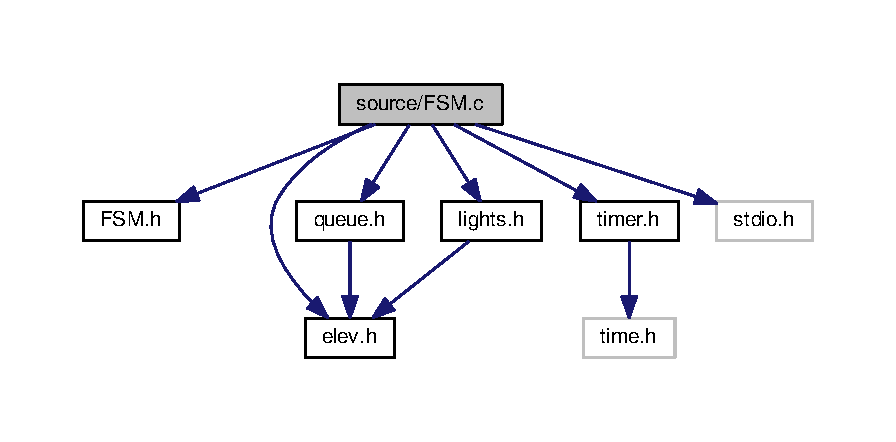
\includegraphics[width=350pt]{FSM_8c__incl}
\end{center}
\end{figure}
\subsection*{Enumerations}
\begin{DoxyCompactItemize}
\item 
enum {\bfseries F\+S\+M\+\_\+states\+\_\+t} \{ {\bfseries F\+L\+O\+O\+R\+\_\+\+C\+L\+O\+S\+ED}, 
{\bfseries F\+L\+O\+O\+R\+\_\+\+O\+P\+EN}, 
{\bfseries M\+O\+V\+I\+NG}, 
{\bfseries S\+T\+A\+T\+I\+O\+N\+A\+RY}
 \}\hypertarget{FSM_8c_a90fb9bfd3b356116f67efce8fe4722a0}{}\label{FSM_8c_a90fb9bfd3b356116f67efce8fe4722a0}

\end{DoxyCompactItemize}
\subsection*{Functions}
\begin{DoxyCompactItemize}
\item 
void \hyperlink{FSM_8c_a28434b3d630ef3dfd0dac8f77fb15700}{F\+S\+M\+\_\+update\+\_\+m\+\_\+pos\+\_\+between} (\hyperlink{elev_8h_a2256dfd58fecce253106f83fd2ed607f}{elev\+\_\+motor\+\_\+direction\+\_\+t} dir, int pos)
\begin{DoxyCompactList}\small\item\em Updates the variable m\+\_\+pos\+\_\+between in order to keep track of which two floors the elevator is currently between. \end{DoxyCompactList}\item 
int \hyperlink{FSM_8c_a5e55d574485ebc87b5d5a74a1a4b35e0}{F\+S\+M\+\_\+system\+\_\+init} ()
\begin{DoxyCompactList}\small\item\em Initializes hardware and leads the elevator to a defined state and position. \end{DoxyCompactList}\item 
void \hyperlink{FSM_8c_a6e0568e2069dc494c5c9014a396b3900}{F\+S\+M\+\_\+state\+\_\+machine} ()\hypertarget{FSM_8c_a6e0568e2069dc494c5c9014a396b3900}{}\label{FSM_8c_a6e0568e2069dc494c5c9014a396b3900}

\begin{DoxyCompactList}\small\item\em Updates current state of the elevator and executes operations accordingly. \end{DoxyCompactList}\end{DoxyCompactItemize}
\subsection*{Variables}
\begin{DoxyCompactItemize}
\item 
static F\+S\+M\+\_\+states\+\_\+t \hyperlink{FSM_8c_aafbb17ec8f22877b3b8ed45d657a85ab}{m\+\_\+current\+\_\+state} = F\+L\+O\+O\+R\+\_\+\+C\+L\+O\+S\+ED\hypertarget{FSM_8c_aafbb17ec8f22877b3b8ed45d657a85ab}{}\label{FSM_8c_aafbb17ec8f22877b3b8ed45d657a85ab}

\begin{DoxyCompactList}\small\item\em The current state of the system. \end{DoxyCompactList}\item 
static \hyperlink{elev_8h_a2256dfd58fecce253106f83fd2ed607f}{elev\+\_\+motor\+\_\+direction\+\_\+t} \hyperlink{FSM_8c_a0a85b6d1e7960e7dbdad8813e26dad6a}{m\+\_\+direction} = D\+I\+R\+N\+\_\+\+S\+T\+OP\hypertarget{FSM_8c_a0a85b6d1e7960e7dbdad8813e26dad6a}{}\label{FSM_8c_a0a85b6d1e7960e7dbdad8813e26dad6a}

\begin{DoxyCompactList}\small\item\em The current direction of the elevator. \end{DoxyCompactList}\item 
static int \hyperlink{FSM_8c_a49746bb03046c26e7ed748ae4704ba8d}{m\+\_\+prev\+\_\+pos} = -\/1\hypertarget{FSM_8c_a49746bb03046c26e7ed748ae4704ba8d}{}\label{FSM_8c_a49746bb03046c26e7ed748ae4704ba8d}

\begin{DoxyCompactList}\small\item\em The previos floor the elevator was located at. 0-\/3 where 0 is the bottom floor and 3 is the top floor. -\/1 is an invalid value. \end{DoxyCompactList}\item 
static int \hyperlink{FSM_8c_a730ab0afd4f7387cc3b2753b60d94498}{m\+\_\+temp\+\_\+pos} = -\/1\hypertarget{FSM_8c_a730ab0afd4f7387cc3b2753b60d94498}{}\label{FSM_8c_a730ab0afd4f7387cc3b2753b60d94498}

\begin{DoxyCompactList}\small\item\em A temporary variable used to avoid reading error from the floor sensors. 0-\/3 where 0 is the bottom floor and 3 is the top floor. -\/1 is an invalid value. \end{DoxyCompactList}\item 
static int \hyperlink{FSM_8c_aa3050385b8dc1c27488abf829fc3a9ca}{m\+\_\+pos\+\_\+between} = 0\hypertarget{FSM_8c_aa3050385b8dc1c27488abf829fc3a9ca}{}\label{FSM_8c_aa3050385b8dc1c27488abf829fc3a9ca}

\begin{DoxyCompactList}\small\item\em Variable used to keep track of wich two floors the elevator is located between as it moves. 1-\/3 where 1 is between floors 1 and 2. \end{DoxyCompactList}\end{DoxyCompactItemize}


\subsection{Detailed Description}
Implementation file for the F\+SM (Finite-\/state machine) module. 



\subsection{Function Documentation}
\index{F\+S\+M.\+c@{F\+S\+M.\+c}!F\+S\+M\+\_\+system\+\_\+init@{F\+S\+M\+\_\+system\+\_\+init}}
\index{F\+S\+M\+\_\+system\+\_\+init@{F\+S\+M\+\_\+system\+\_\+init}!F\+S\+M.\+c@{F\+S\+M.\+c}}
\subsubsection[{\texorpdfstring{F\+S\+M\+\_\+system\+\_\+init()}{FSM_system_init()}}]{\setlength{\rightskip}{0pt plus 5cm}int F\+S\+M\+\_\+system\+\_\+init (
\begin{DoxyParamCaption}
{}
\end{DoxyParamCaption}
)}\hypertarget{FSM_8c_a5e55d574485ebc87b5d5a74a1a4b35e0}{}\label{FSM_8c_a5e55d574485ebc87b5d5a74a1a4b35e0}


Initializes hardware and leads the elevator to a defined state and position. 

\begin{DoxyReturn}{Returns}
0 if the elevator hardware is unable to initialize, 1 otherwise. 
\end{DoxyReturn}


Definition at line 65 of file F\+S\+M.\+c.

\index{F\+S\+M.\+c@{F\+S\+M.\+c}!F\+S\+M\+\_\+update\+\_\+m\+\_\+pos\+\_\+between@{F\+S\+M\+\_\+update\+\_\+m\+\_\+pos\+\_\+between}}
\index{F\+S\+M\+\_\+update\+\_\+m\+\_\+pos\+\_\+between@{F\+S\+M\+\_\+update\+\_\+m\+\_\+pos\+\_\+between}!F\+S\+M.\+c@{F\+S\+M.\+c}}
\subsubsection[{\texorpdfstring{F\+S\+M\+\_\+update\+\_\+m\+\_\+pos\+\_\+between(elev\+\_\+motor\+\_\+direction\+\_\+t dir, int pos)}{FSM_update_m_pos_between(elev_motor_direction_t dir, int pos)}}]{\setlength{\rightskip}{0pt plus 5cm}void F\+S\+M\+\_\+update\+\_\+m\+\_\+pos\+\_\+between (
\begin{DoxyParamCaption}
\item[{{\bf elev\+\_\+motor\+\_\+direction\+\_\+t}}]{dir, }
\item[{int}]{pos}
\end{DoxyParamCaption}
)}\hypertarget{FSM_8c_a28434b3d630ef3dfd0dac8f77fb15700}{}\label{FSM_8c_a28434b3d630ef3dfd0dac8f77fb15700}


Updates the variable m\+\_\+pos\+\_\+between in order to keep track of which two floors the elevator is currently between. 


\begin{DoxyParams}[1]{Parameters}
\mbox{\tt in}  & {\em dir} & The current direction of the elevator\\
\hline
\mbox{\tt in}  & {\em pos} & The previos floor the elevator was located at\\
\hline
\end{DoxyParams}
\begin{DoxyReturn}{Returns}
A number 1-\/3 representing the three possible areas between the floors 
\end{DoxyReturn}


Definition at line 184 of file F\+S\+M.\+c.


\hypertarget{FSM_8h}{}\section{source/\+F\+SM.h File Reference}
\label{FSM_8h}\index{source/\+F\+S\+M.\+h@{source/\+F\+S\+M.\+h}}


A library containing functions regarding the F\+SM (Finite-\/state machine) module.  


This graph shows which files directly or indirectly include this file\+:
\nopagebreak
\begin{figure}[H]
\begin{center}
\leavevmode
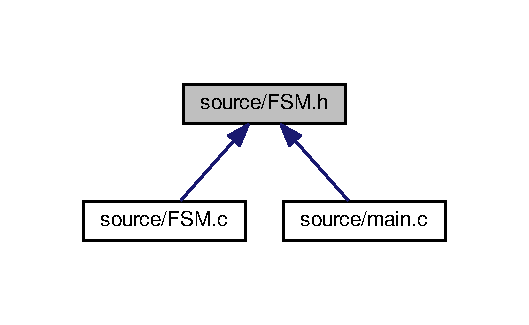
\includegraphics[width=254pt]{FSM_8h__dep__incl}
\end{center}
\end{figure}
\subsection*{Functions}
\begin{DoxyCompactItemize}
\item 
void \hyperlink{FSM_8h_a6e0568e2069dc494c5c9014a396b3900}{F\+S\+M\+\_\+state\+\_\+machine} ()\hypertarget{FSM_8h_a6e0568e2069dc494c5c9014a396b3900}{}\label{FSM_8h_a6e0568e2069dc494c5c9014a396b3900}

\begin{DoxyCompactList}\small\item\em Updates current state of the elevator and executes operations accordingly. \end{DoxyCompactList}\item 
int \hyperlink{FSM_8h_a5e55d574485ebc87b5d5a74a1a4b35e0}{F\+S\+M\+\_\+system\+\_\+init} ()
\begin{DoxyCompactList}\small\item\em Initializes hardware and leads the elevator to a defined state and position. \end{DoxyCompactList}\end{DoxyCompactItemize}


\subsection{Detailed Description}
A library containing functions regarding the F\+SM (Finite-\/state machine) module. 



\subsection{Function Documentation}
\index{F\+S\+M.\+h@{F\+S\+M.\+h}!F\+S\+M\+\_\+system\+\_\+init@{F\+S\+M\+\_\+system\+\_\+init}}
\index{F\+S\+M\+\_\+system\+\_\+init@{F\+S\+M\+\_\+system\+\_\+init}!F\+S\+M.\+h@{F\+S\+M.\+h}}
\subsubsection[{\texorpdfstring{F\+S\+M\+\_\+system\+\_\+init()}{FSM_system_init()}}]{\setlength{\rightskip}{0pt plus 5cm}int F\+S\+M\+\_\+system\+\_\+init (
\begin{DoxyParamCaption}
{}
\end{DoxyParamCaption}
)}\hypertarget{FSM_8h_a5e55d574485ebc87b5d5a74a1a4b35e0}{}\label{FSM_8h_a5e55d574485ebc87b5d5a74a1a4b35e0}


Initializes hardware and leads the elevator to a defined state and position. 

\begin{DoxyReturn}{Returns}
0 if the elevator hardware is unable to initialize, 1 otherwise. 
\end{DoxyReturn}


Definition at line 46 of file F\+S\+M.\+c.


\hypertarget{io_8c}{}\section{source/io.c File Reference}
\label{io_8c}\index{source/io.\+c@{source/io.\+c}}


Implementation file regarding the io (in/out) module.  


{\ttfamily \#include \char`\"{}io.\+h\char`\"{}}\\*
{\ttfamily \#include \char`\"{}channels.\+h\char`\"{}}\\*
{\ttfamily \#include $<$comedilib.\+h$>$}\\*
Include dependency graph for io.\+c\+:
\nopagebreak
\begin{figure}[H]
\begin{center}
\leavevmode
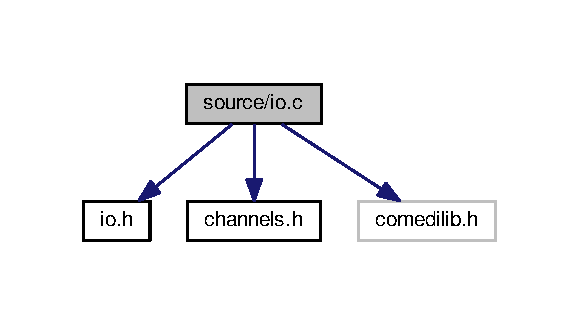
\includegraphics[width=278pt]{io_8c__incl}
\end{center}
\end{figure}
\subsection*{Functions}
\begin{DoxyCompactItemize}
\item 
int \hyperlink{io_8c_a12ce98b64f2019ac45b44826a4db7ec9}{io\+\_\+init} ()
\item 
void \hyperlink{io_8c_a4d538858b80ee856217e3ecfde8a3c60}{io\+\_\+set\+\_\+bit} (int channel)
\item 
void \hyperlink{io_8c_a97951257634a0778b858a4ced7558f81}{io\+\_\+clear\+\_\+bit} (int channel)
\item 
void \hyperlink{io_8c_a1c2c5df63111187109ef11be354621bd}{io\+\_\+write\+\_\+analog} (int channel, int value)
\item 
int \hyperlink{io_8c_ae9e08ee7d41b07b153e2ddaae4dc53cb}{io\+\_\+read\+\_\+bit} (int channel)
\item 
int \hyperlink{io_8c_ab145a5637d2c463dfb5741e1a748dd74}{io\+\_\+read\+\_\+analog} (int channel)
\end{DoxyCompactItemize}


\subsection{Detailed Description}
Implementation file regarding the io (in/out) module. 



\subsection{Function Documentation}
\index{io.\+c@{io.\+c}!io\+\_\+clear\+\_\+bit@{io\+\_\+clear\+\_\+bit}}
\index{io\+\_\+clear\+\_\+bit@{io\+\_\+clear\+\_\+bit}!io.\+c@{io.\+c}}
\subsubsection[{\texorpdfstring{io\+\_\+clear\+\_\+bit(int channel)}{io_clear_bit(int channel)}}]{\setlength{\rightskip}{0pt plus 5cm}void io\+\_\+clear\+\_\+bit (
\begin{DoxyParamCaption}
\item[{int}]{channel}
\end{DoxyParamCaption}
)}\hypertarget{io_8c_a97951257634a0778b858a4ced7558f81}{}\label{io_8c_a97951257634a0778b858a4ced7558f81}
Clears a digital channel bit. 
\begin{DoxyParams}{Parameters}
{\em channel} & Channel bit to set. \\
\hline
\end{DoxyParams}


Definition at line 51 of file io.\+c.

\index{io.\+c@{io.\+c}!io\+\_\+init@{io\+\_\+init}}
\index{io\+\_\+init@{io\+\_\+init}!io.\+c@{io.\+c}}
\subsubsection[{\texorpdfstring{io\+\_\+init()}{io_init()}}]{\setlength{\rightskip}{0pt plus 5cm}int io\+\_\+init (
\begin{DoxyParamCaption}
{}
\end{DoxyParamCaption}
)}\hypertarget{io_8c_a12ce98b64f2019ac45b44826a4db7ec9}{}\label{io_8c_a12ce98b64f2019ac45b44826a4db7ec9}
Initialize lib\+Comedi in \char`\"{}\+Sanntidssalen\char`\"{} \begin{DoxyReturn}{Returns}
Non-\/zero on success and 0 on failure 
\end{DoxyReturn}


Definition at line 24 of file io.\+c.

\index{io.\+c@{io.\+c}!io\+\_\+read\+\_\+analog@{io\+\_\+read\+\_\+analog}}
\index{io\+\_\+read\+\_\+analog@{io\+\_\+read\+\_\+analog}!io.\+c@{io.\+c}}
\subsubsection[{\texorpdfstring{io\+\_\+read\+\_\+analog(int channel)}{io_read_analog(int channel)}}]{\setlength{\rightskip}{0pt plus 5cm}int io\+\_\+read\+\_\+analog (
\begin{DoxyParamCaption}
\item[{int}]{channel}
\end{DoxyParamCaption}
)}\hypertarget{io_8c_ab145a5637d2c463dfb5741e1a748dd74}{}\label{io_8c_ab145a5637d2c463dfb5741e1a748dd74}
Reads a bit value from an analog channel. 
\begin{DoxyParams}{Parameters}
{\em channel} & Channel to read from. \\
\hline
\end{DoxyParams}
\begin{DoxyReturn}{Returns}
Value read. 
\end{DoxyReturn}


Definition at line 72 of file io.\+c.

\index{io.\+c@{io.\+c}!io\+\_\+read\+\_\+bit@{io\+\_\+read\+\_\+bit}}
\index{io\+\_\+read\+\_\+bit@{io\+\_\+read\+\_\+bit}!io.\+c@{io.\+c}}
\subsubsection[{\texorpdfstring{io\+\_\+read\+\_\+bit(int channel)}{io_read_bit(int channel)}}]{\setlength{\rightskip}{0pt plus 5cm}int io\+\_\+read\+\_\+bit (
\begin{DoxyParamCaption}
\item[{int}]{channel}
\end{DoxyParamCaption}
)}\hypertarget{io_8c_ae9e08ee7d41b07b153e2ddaae4dc53cb}{}\label{io_8c_ae9e08ee7d41b07b153e2ddaae4dc53cb}
Reads a bit value from a digital channel. 
\begin{DoxyParams}{Parameters}
{\em channel} & Channel to read from. \\
\hline
\end{DoxyParams}
\begin{DoxyReturn}{Returns}
Value read. 
\end{DoxyReturn}


Definition at line 63 of file io.\+c.

\index{io.\+c@{io.\+c}!io\+\_\+set\+\_\+bit@{io\+\_\+set\+\_\+bit}}
\index{io\+\_\+set\+\_\+bit@{io\+\_\+set\+\_\+bit}!io.\+c@{io.\+c}}
\subsubsection[{\texorpdfstring{io\+\_\+set\+\_\+bit(int channel)}{io_set_bit(int channel)}}]{\setlength{\rightskip}{0pt plus 5cm}void io\+\_\+set\+\_\+bit (
\begin{DoxyParamCaption}
\item[{int}]{channel}
\end{DoxyParamCaption}
)}\hypertarget{io_8c_a4d538858b80ee856217e3ecfde8a3c60}{}\label{io_8c_a4d538858b80ee856217e3ecfde8a3c60}
Sets a digital channel bit. 
\begin{DoxyParams}{Parameters}
{\em channel} & Channel bit to set. \\
\hline
\end{DoxyParams}


Definition at line 45 of file io.\+c.

\index{io.\+c@{io.\+c}!io\+\_\+write\+\_\+analog@{io\+\_\+write\+\_\+analog}}
\index{io\+\_\+write\+\_\+analog@{io\+\_\+write\+\_\+analog}!io.\+c@{io.\+c}}
\subsubsection[{\texorpdfstring{io\+\_\+write\+\_\+analog(int channel, int value)}{io_write_analog(int channel, int value)}}]{\setlength{\rightskip}{0pt plus 5cm}void io\+\_\+write\+\_\+analog (
\begin{DoxyParamCaption}
\item[{int}]{channel, }
\item[{int}]{value}
\end{DoxyParamCaption}
)}\hypertarget{io_8c_a1c2c5df63111187109ef11be354621bd}{}\label{io_8c_a1c2c5df63111187109ef11be354621bd}
Writes a value to an analog channel. 
\begin{DoxyParams}{Parameters}
{\em channel} & Channel to write to. \\
\hline
{\em value} & Value to write. \\
\hline
\end{DoxyParams}


Definition at line 57 of file io.\+c.


\hypertarget{io_8h}{}\section{source/io.h File Reference}
\label{io_8h}\index{source/io.\+h@{source/io.\+h}}


A library containing functions regarding the io (in/out) module.  


This graph shows which files directly or indirectly include this file\+:
% FIG 0
\subsection*{Functions}
\begin{DoxyCompactItemize}
\item 
int \hyperlink{io_8h_a12ce98b64f2019ac45b44826a4db7ec9}{io\+\_\+init} ()
\item 
void \hyperlink{io_8h_a4d538858b80ee856217e3ecfde8a3c60}{io\+\_\+set\+\_\+bit} (int channel)
\item 
void \hyperlink{io_8h_a97951257634a0778b858a4ced7558f81}{io\+\_\+clear\+\_\+bit} (int channel)
\item 
void \hyperlink{io_8h_a1c2c5df63111187109ef11be354621bd}{io\+\_\+write\+\_\+analog} (int channel, int value)
\item 
int \hyperlink{io_8h_ae9e08ee7d41b07b153e2ddaae4dc53cb}{io\+\_\+read\+\_\+bit} (int channel)
\item 
int \hyperlink{io_8h_ab145a5637d2c463dfb5741e1a748dd74}{io\+\_\+read\+\_\+analog} (int channel)
\end{DoxyCompactItemize}


\subsection{Detailed Description}
A library containing functions regarding the io (in/out) module. 



\subsection{Function Documentation}
\index{io.\+h@{io.\+h}!io\+\_\+clear\+\_\+bit@{io\+\_\+clear\+\_\+bit}}
\index{io\+\_\+clear\+\_\+bit@{io\+\_\+clear\+\_\+bit}!io.\+h@{io.\+h}}
\subsubsection[{\texorpdfstring{io\+\_\+clear\+\_\+bit(int channel)}{io_clear_bit(int channel)}}]{\setlength{\rightskip}{0pt plus 5cm}void io\+\_\+clear\+\_\+bit (
\begin{DoxyParamCaption}
\item[{int}]{channel}
\end{DoxyParamCaption}
)}\hypertarget{io_8h_a97951257634a0778b858a4ced7558f81}{}\label{io_8h_a97951257634a0778b858a4ced7558f81}
Clears a digital channel bit. 
\begin{DoxyParams}{Parameters}
{\em channel} & Channel bit to set. \\
\hline
\end{DoxyParams}


Definition at line 45 of file io.\+c.

\index{io.\+h@{io.\+h}!io\+\_\+init@{io\+\_\+init}}
\index{io\+\_\+init@{io\+\_\+init}!io.\+h@{io.\+h}}
\subsubsection[{\texorpdfstring{io\+\_\+init()}{io_init()}}]{\setlength{\rightskip}{0pt plus 5cm}int io\+\_\+init (
\begin{DoxyParamCaption}
{}
\end{DoxyParamCaption}
)}\hypertarget{io_8h_a12ce98b64f2019ac45b44826a4db7ec9}{}\label{io_8h_a12ce98b64f2019ac45b44826a4db7ec9}
Initialize lib\+Comedi in \char`\"{}\+Sanntidssalen\char`\"{} \begin{DoxyReturn}{Returns}
Non-\/zero on success and 0 on failure 
\end{DoxyReturn}


Definition at line 18 of file io.\+c.

\index{io.\+h@{io.\+h}!io\+\_\+read\+\_\+analog@{io\+\_\+read\+\_\+analog}}
\index{io\+\_\+read\+\_\+analog@{io\+\_\+read\+\_\+analog}!io.\+h@{io.\+h}}
\subsubsection[{\texorpdfstring{io\+\_\+read\+\_\+analog(int channel)}{io_read_analog(int channel)}}]{\setlength{\rightskip}{0pt plus 5cm}int io\+\_\+read\+\_\+analog (
\begin{DoxyParamCaption}
\item[{int}]{channel}
\end{DoxyParamCaption}
)}\hypertarget{io_8h_ab145a5637d2c463dfb5741e1a748dd74}{}\label{io_8h_ab145a5637d2c463dfb5741e1a748dd74}
Reads a bit value from an analog channel. 
\begin{DoxyParams}{Parameters}
{\em channel} & Channel to read from. \\
\hline
\end{DoxyParams}
\begin{DoxyReturn}{Returns}
Value read. 
\end{DoxyReturn}


Definition at line 66 of file io.\+c.

\index{io.\+h@{io.\+h}!io\+\_\+read\+\_\+bit@{io\+\_\+read\+\_\+bit}}
\index{io\+\_\+read\+\_\+bit@{io\+\_\+read\+\_\+bit}!io.\+h@{io.\+h}}
\subsubsection[{\texorpdfstring{io\+\_\+read\+\_\+bit(int channel)}{io_read_bit(int channel)}}]{\setlength{\rightskip}{0pt plus 5cm}int io\+\_\+read\+\_\+bit (
\begin{DoxyParamCaption}
\item[{int}]{channel}
\end{DoxyParamCaption}
)}\hypertarget{io_8h_ae9e08ee7d41b07b153e2ddaae4dc53cb}{}\label{io_8h_ae9e08ee7d41b07b153e2ddaae4dc53cb}
Reads a bit value from a digital channel. 
\begin{DoxyParams}{Parameters}
{\em channel} & Channel to read from. \\
\hline
\end{DoxyParams}
\begin{DoxyReturn}{Returns}
Value read. 
\end{DoxyReturn}


Definition at line 57 of file io.\+c.

\index{io.\+h@{io.\+h}!io\+\_\+set\+\_\+bit@{io\+\_\+set\+\_\+bit}}
\index{io\+\_\+set\+\_\+bit@{io\+\_\+set\+\_\+bit}!io.\+h@{io.\+h}}
\subsubsection[{\texorpdfstring{io\+\_\+set\+\_\+bit(int channel)}{io_set_bit(int channel)}}]{\setlength{\rightskip}{0pt plus 5cm}void io\+\_\+set\+\_\+bit (
\begin{DoxyParamCaption}
\item[{int}]{channel}
\end{DoxyParamCaption}
)}\hypertarget{io_8h_a4d538858b80ee856217e3ecfde8a3c60}{}\label{io_8h_a4d538858b80ee856217e3ecfde8a3c60}
Sets a digital channel bit. 
\begin{DoxyParams}{Parameters}
{\em channel} & Channel bit to set. \\
\hline
\end{DoxyParams}


Definition at line 39 of file io.\+c.

\index{io.\+h@{io.\+h}!io\+\_\+write\+\_\+analog@{io\+\_\+write\+\_\+analog}}
\index{io\+\_\+write\+\_\+analog@{io\+\_\+write\+\_\+analog}!io.\+h@{io.\+h}}
\subsubsection[{\texorpdfstring{io\+\_\+write\+\_\+analog(int channel, int value)}{io_write_analog(int channel, int value)}}]{\setlength{\rightskip}{0pt plus 5cm}void io\+\_\+write\+\_\+analog (
\begin{DoxyParamCaption}
\item[{int}]{channel, }
\item[{int}]{value}
\end{DoxyParamCaption}
)}\hypertarget{io_8h_a1c2c5df63111187109ef11be354621bd}{}\label{io_8h_a1c2c5df63111187109ef11be354621bd}
Writes a value to an analog channel. 
\begin{DoxyParams}{Parameters}
{\em channel} & Channel to write to. \\
\hline
{\em value} & Value to write. \\
\hline
\end{DoxyParams}


Definition at line 51 of file io.\+c.


\hypertarget{lights_8c}{}\section{source/lights.c File Reference}
\label{lights_8c}\index{source/lights.\+c@{source/lights.\+c}}


Implentation file regarding the lights module.  


{\ttfamily \#include \char`\"{}lights.\+h\char`\"{}}\\*
Include dependency graph for lights.\+c\+:
\nopagebreak
\begin{figure}[H]
\begin{center}
\leavevmode
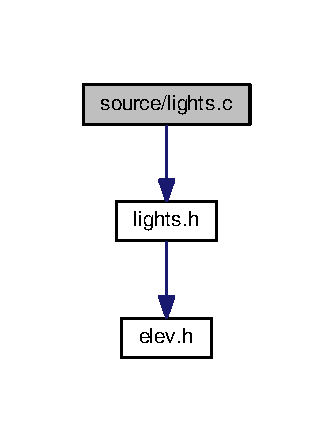
\includegraphics[width=160pt]{lights_8c__incl}
\end{center}
\end{figure}
\subsection*{Functions}
\begin{DoxyCompactItemize}
\item 
void \hyperlink{lights_8c_add63f7837141be6313f3ea649a219334}{lights\+\_\+set\+\_\+ordering\+\_\+lights\+\_\+command} ()\hypertarget{lights_8c_add63f7837141be6313f3ea649a219334}{}\label{lights_8c_add63f7837141be6313f3ea649a219334}

\begin{DoxyCompactList}\small\item\em Checks the signal from the command buttons and sets the value at the corresponding position in the array \char`\"{}lights\char`\"{} to 1. \end{DoxyCompactList}\item 
void \hyperlink{lights_8c_a521fc236d5cd04d9d0c9c6cc2047881e}{lights\+\_\+set\+\_\+ordering\+\_\+lights\+\_\+up} ()\hypertarget{lights_8c_a521fc236d5cd04d9d0c9c6cc2047881e}{}\label{lights_8c_a521fc236d5cd04d9d0c9c6cc2047881e}

\begin{DoxyCompactList}\small\item\em Checks the signal from the up buttons and sets the value at the corresponding position in the array \char`\"{}lights\char`\"{} to 1. \end{DoxyCompactList}\item 
void \hyperlink{lights_8c_a8cd744900f1d35427f3a8a8deb39f9a9}{lights\+\_\+set\+\_\+ordering\+\_\+lights\+\_\+down} ()\hypertarget{lights_8c_a8cd744900f1d35427f3a8a8deb39f9a9}{}\label{lights_8c_a8cd744900f1d35427f3a8a8deb39f9a9}

\begin{DoxyCompactList}\small\item\em Checks the signal from the down buttons and sets the value at the corresponding position in the array \char`\"{}lights\char`\"{} to 1. \end{DoxyCompactList}\item 
void \hyperlink{lights_8c_ab9fdad0624f78e12a34b9aed0e501604}{lights\+\_\+set\+\_\+ordering\+\_\+lights\+\_\+array} ()\hypertarget{lights_8c_ab9fdad0624f78e12a34b9aed0e501604}{}\label{lights_8c_ab9fdad0624f78e12a34b9aed0e501604}

\begin{DoxyCompactList}\small\item\em Gets signal from ordering button, and sets the corresponding element in the \char`\"{}lights\char`\"{} array to 1. \end{DoxyCompactList}\item 
void \hyperlink{lights_8c_a9581cca0e3b21bb9db5d4dac1f5d04fd}{lights\+\_\+reset\+\_\+ordering\+\_\+lights\+\_\+array} (int floor)
\begin{DoxyCompactList}\small\item\em Sets the values in the array \char`\"{}lights\char`\"{} for the ordering lights to the corresponding floor to 0. \end{DoxyCompactList}\item 
void \hyperlink{lights_8c_ab9e40612b431e6952a2b51b6b20c6843}{lights\+\_\+reset\+\_\+all\+\_\+ordering\+\_\+lights\+\_\+array} ()\hypertarget{lights_8c_ab9e40612b431e6952a2b51b6b20c6843}{}\label{lights_8c_ab9e40612b431e6952a2b51b6b20c6843}

\begin{DoxyCompactList}\small\item\em Sets all the values in the array \char`\"{}lights\char`\"{} to 0. \end{DoxyCompactList}\item 
void \hyperlink{lights_8c_af2210991bdfe739662bce1dd46388d27}{lights\+\_\+update\+\_\+ordering\+\_\+lights} ()\hypertarget{lights_8c_af2210991bdfe739662bce1dd46388d27}{}\label{lights_8c_af2210991bdfe739662bce1dd46388d27}

\begin{DoxyCompactList}\small\item\em Updates the ordering lights, on or off, according to the array \char`\"{}lights\char`\"{}. \end{DoxyCompactList}\end{DoxyCompactItemize}
\subsection*{Variables}
\begin{DoxyCompactItemize}
\item 
const int {\bfseries L\+I\+G\+H\+T\+\_\+\+S\+I\+ZE} = 10\hypertarget{lights_8c_a956164e83fbf9605989ef9d7a4b4b784}{}\label{lights_8c_a956164e83fbf9605989ef9d7a4b4b784}

\end{DoxyCompactItemize}


\subsection{Detailed Description}
Implentation file regarding the lights module. 



\subsection{Function Documentation}
\index{lights.\+c@{lights.\+c}!lights\+\_\+reset\+\_\+ordering\+\_\+lights\+\_\+array@{lights\+\_\+reset\+\_\+ordering\+\_\+lights\+\_\+array}}
\index{lights\+\_\+reset\+\_\+ordering\+\_\+lights\+\_\+array@{lights\+\_\+reset\+\_\+ordering\+\_\+lights\+\_\+array}!lights.\+c@{lights.\+c}}
\subsubsection[{\texorpdfstring{lights\+\_\+reset\+\_\+ordering\+\_\+lights\+\_\+array(int floor)}{lights_reset_ordering_lights_array(int floor)}}]{\setlength{\rightskip}{0pt plus 5cm}void lights\+\_\+reset\+\_\+ordering\+\_\+lights\+\_\+array (
\begin{DoxyParamCaption}
\item[{int}]{floor}
\end{DoxyParamCaption}
)}\hypertarget{lights_8c_a9581cca0e3b21bb9db5d4dac1f5d04fd}{}\label{lights_8c_a9581cca0e3b21bb9db5d4dac1f5d04fd}


Sets the values in the array \char`\"{}lights\char`\"{} for the ordering lights to the corresponding floor to 0. 


\begin{DoxyParams}[1]{Parameters}
\mbox{\tt in}  & {\em floor} & The floor where the ordering lights will be turned off. Must be an integer in range 0-\/3. \\
\hline
\end{DoxyParams}


Definition at line 39 of file lights.\+c.


\hypertarget{lights_8h}{}\section{source/lights.h File Reference}
\label{lights_8h}\index{source/lights.\+h@{source/lights.\+h}}


A library containing the functions regarding the lights module.  


{\ttfamily \#include \char`\"{}elev.\+h\char`\"{}}\\*
Include dependency graph for lights.\+h\+:\nopagebreak
\begin{figure}[H]
\begin{center}
\leavevmode
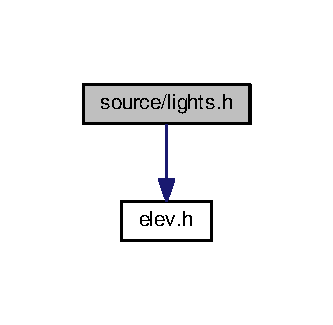
\includegraphics[width=160pt]{lights_8h__incl}
\end{center}
\end{figure}
This graph shows which files directly or indirectly include this file\+:\nopagebreak
\begin{figure}[H]
\begin{center}
\leavevmode
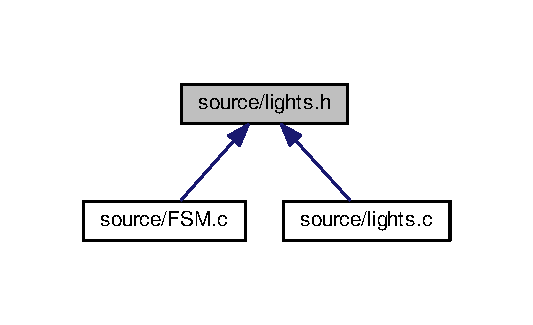
\includegraphics[width=256pt]{lights_8h__dep__incl}
\end{center}
\end{figure}
\subsection*{Functions}
\begin{DoxyCompactItemize}
\item 
void \hyperlink{lights_8h_af2210991bdfe739662bce1dd46388d27}{lights\+\_\+update\+\_\+ordering\+\_\+lights} ()\hypertarget{lights_8h_af2210991bdfe739662bce1dd46388d27}{}\label{lights_8h_af2210991bdfe739662bce1dd46388d27}

\begin{DoxyCompactList}\small\item\em Updates the ordering lights, on or off, according to the array \char`\"{}lights\char`\"{}. \end{DoxyCompactList}\item 
void \hyperlink{lights_8h_a9581cca0e3b21bb9db5d4dac1f5d04fd}{lights\+\_\+reset\+\_\+ordering\+\_\+lights\+\_\+array} (int floor)
\begin{DoxyCompactList}\small\item\em Sets the values in the array \char`\"{}lights\char`\"{} for the ordering lights to the corresponding floor to 0. \end{DoxyCompactList}\item 
void \hyperlink{lights_8h_ab9e40612b431e6952a2b51b6b20c6843}{lights\+\_\+reset\+\_\+all\+\_\+ordering\+\_\+lights\+\_\+array} ()\hypertarget{lights_8h_ab9e40612b431e6952a2b51b6b20c6843}{}\label{lights_8h_ab9e40612b431e6952a2b51b6b20c6843}

\begin{DoxyCompactList}\small\item\em Sets all the values in the array \char`\"{}lights\char`\"{} to 0. \end{DoxyCompactList}\item 
void \hyperlink{lights_8h_ab9fdad0624f78e12a34b9aed0e501604}{lights\+\_\+set\+\_\+ordering\+\_\+lights\+\_\+array} ()\hypertarget{lights_8h_ab9fdad0624f78e12a34b9aed0e501604}{}\label{lights_8h_ab9fdad0624f78e12a34b9aed0e501604}

\begin{DoxyCompactList}\small\item\em Gets signal from ordering button, and sets the corresponding element in the \char`\"{}lights\char`\"{} array to 1. \end{DoxyCompactList}\end{DoxyCompactItemize}


\subsection{Detailed Description}
A library containing the functions regarding the lights module. 



\subsection{Function Documentation}
\index{lights.\+h@{lights.\+h}!lights\+\_\+reset\+\_\+ordering\+\_\+lights\+\_\+array@{lights\+\_\+reset\+\_\+ordering\+\_\+lights\+\_\+array}}
\index{lights\+\_\+reset\+\_\+ordering\+\_\+lights\+\_\+array@{lights\+\_\+reset\+\_\+ordering\+\_\+lights\+\_\+array}!lights.\+h@{lights.\+h}}
\subsubsection[{\texorpdfstring{lights\+\_\+reset\+\_\+ordering\+\_\+lights\+\_\+array(int floor)}{lights_reset_ordering_lights_array(int floor)}}]{\setlength{\rightskip}{0pt plus 5cm}void lights\+\_\+reset\+\_\+ordering\+\_\+lights\+\_\+array (
\begin{DoxyParamCaption}
\item[{int}]{floor}
\end{DoxyParamCaption}
)}\hypertarget{lights_8h_a9581cca0e3b21bb9db5d4dac1f5d04fd}{}\label{lights_8h_a9581cca0e3b21bb9db5d4dac1f5d04fd}


Sets the values in the array \char`\"{}lights\char`\"{} for the ordering lights to the corresponding floor to 0. 


\begin{DoxyParams}[1]{Parameters}
\mbox{\tt in}  & {\em floor} & The floor where the ordering lights will be turned off. Must be an integer in range 0-\/3. \\
\hline
\end{DoxyParams}


Definition at line 46 of file lights.\+c.


\hypertarget{main_8c}{}\section{source/main.c File Reference}
\label{main_8c}\index{source/main.\+c@{source/main.\+c}}


File for the main function of the program.  


{\ttfamily \#include \char`\"{}F\+S\+M.\+h\char`\"{}}\\*
{\ttfamily \#include $<$stdio.\+h$>$}\\*
Include dependency graph for main.\+c\+:
% FIG 0
\subsection*{Functions}
\begin{DoxyCompactItemize}
\item 
int {\bfseries main} ()\hypertarget{main_8c_ae66f6b31b5ad750f1fe042a706a4e3d4}{}\label{main_8c_ae66f6b31b5ad750f1fe042a706a4e3d4}

\end{DoxyCompactItemize}


\subsection{Detailed Description}
File for the main function of the program. 


\hypertarget{queue_8c}{}\section{source/queue.c File Reference}
\label{queue_8c}\index{source/queue.\+c@{source/queue.\+c}}


Implementation file for the queue module.  


{\ttfamily \#include \char`\"{}queue.\+h\char`\"{}}\\*
{\ttfamily \#include $<$stdlib.\+h$>$}\\*
Include dependency graph for queue.\+c\+:
% FIG 0
\subsection*{Functions}
\begin{DoxyCompactItemize}
\item 
int {\bfseries queue\+\_\+check\+\_\+if\+\_\+order\+\_\+above} (int pos)\hypertarget{queue_8c_a94cf2844e2284f6732aee540f4449e6e}{}\label{queue_8c_a94cf2844e2284f6732aee540f4449e6e}

\item 
int {\bfseries queue\+\_\+check\+\_\+if\+\_\+order\+\_\+below} (int pos)\hypertarget{queue_8c_a1ca9b544e437207202f8220247e91623}{}\label{queue_8c_a1ca9b544e437207202f8220247e91623}

\item 
void {\bfseries queue\+\_\+set\+\_\+order\+\_\+commands} ()\hypertarget{queue_8c_aa7a44ff846c59512087ceb229f23b04d}{}\label{queue_8c_aa7a44ff846c59512087ceb229f23b04d}

\item 
void {\bfseries queue\+\_\+set\+\_\+order\+\_\+up} ()\hypertarget{queue_8c_a818221e86567bbe51f27f44b4b545cbc}{}\label{queue_8c_a818221e86567bbe51f27f44b4b545cbc}

\item 
void {\bfseries queue\+\_\+set\+\_\+order\+\_\+down} ()\hypertarget{queue_8c_a1e1c8dc89a2ca02c5cc337edb8640ab9}{}\label{queue_8c_a1e1c8dc89a2ca02c5cc337edb8640ab9}

\item 
void \hyperlink{queue_8c_a35a940db362073d0e6f2de5c98ca8642}{queue\+\_\+take\+\_\+order} ()\hypertarget{queue_8c_a35a940db362073d0e6f2de5c98ca8642}{}\label{queue_8c_a35a940db362073d0e6f2de5c98ca8642}

\begin{DoxyCompactList}\small\item\em Sets the value in the array \char`\"{}orders\char`\"{} to the corresponding order to 1. \end{DoxyCompactList}\item 
int \hyperlink{queue_8c_a8db0e454b9930c5cd767d158d9e46ebc}{queue\+\_\+get\+\_\+order} (int floor)
\begin{DoxyCompactList}\small\item\em Checks if there are any orders to given floor. \end{DoxyCompactList}\item 
void \hyperlink{queue_8c_af136c602c4abb11df25cf6e362407e0f}{queue\+\_\+delete\+\_\+order} (int floor)
\begin{DoxyCompactList}\small\item\em Sets the value in the array \char`\"{}orders\char`\"{} to the corresponding order to 0. \end{DoxyCompactList}\item 
void \hyperlink{queue_8c_a25ddb5a68fbbd63e2ceb905b3c57595f}{queue\+\_\+delete\+\_\+all\+\_\+orders} ()\hypertarget{queue_8c_a25ddb5a68fbbd63e2ceb905b3c57595f}{}\label{queue_8c_a25ddb5a68fbbd63e2ceb905b3c57595f}

\begin{DoxyCompactList}\small\item\em Sets all values in the array \char`\"{}orders\char`\"{} to 0. \end{DoxyCompactList}\item 
\hyperlink{elev_8h_a2256dfd58fecce253106f83fd2ed607f}{elev\+\_\+motor\+\_\+direction\+\_\+t} \hyperlink{queue_8c_ae1318c7bf5c2321a99432394e0cf4515}{queue\+\_\+calculate\+\_\+direction} (\hyperlink{elev_8h_a2256dfd58fecce253106f83fd2ed607f}{elev\+\_\+motor\+\_\+direction\+\_\+t} prev\+\_\+dir, int pos, int pos\+\_\+between)
\begin{DoxyCompactList}\small\item\em Calculates the elevator\textquotesingle{}s next direction. \end{DoxyCompactList}\item 
int \hyperlink{queue_8c_a9bda618087afe5dc6c669643b2628537}{queue\+\_\+should\+\_\+stop\+\_\+at\+\_\+floor} (\hyperlink{elev_8h_a2256dfd58fecce253106f83fd2ed607f}{elev\+\_\+motor\+\_\+direction\+\_\+t} motor\+\_\+dir, int floor)
\begin{DoxyCompactList}\small\item\em Checks if the elevator should stop at the given floor. \end{DoxyCompactList}\item 
int \hyperlink{queue_8c_a03cce911f28d999c0647e7ce9e928ff9}{queue\+\_\+have\+\_\+orders} ()
\begin{DoxyCompactList}\small\item\em Checks if there are any orders. \end{DoxyCompactList}\end{DoxyCompactItemize}
\subsection*{Variables}
\begin{DoxyCompactItemize}
\item 
const int {\bfseries O\+R\+D\+E\+R\+\_\+\+S\+I\+ZE} = 10\hypertarget{queue_8c_a8b39957d8636cc75a159ab478ec0bcc5}{}\label{queue_8c_a8b39957d8636cc75a159ab478ec0bcc5}

\end{DoxyCompactItemize}


\subsection{Detailed Description}
Implementation file for the queue module. 



\subsection{Function Documentation}
\index{queue.\+c@{queue.\+c}!queue\+\_\+calculate\+\_\+direction@{queue\+\_\+calculate\+\_\+direction}}
\index{queue\+\_\+calculate\+\_\+direction@{queue\+\_\+calculate\+\_\+direction}!queue.\+c@{queue.\+c}}
\subsubsection[{\texorpdfstring{queue\+\_\+calculate\+\_\+direction(elev\+\_\+motor\+\_\+direction\+\_\+t prev\+\_\+dir, int pos, int pos\+\_\+between)}{queue_calculate_direction(elev_motor_direction_t prev_dir, int pos, int pos_between)}}]{\setlength{\rightskip}{0pt plus 5cm}{\bf elev\+\_\+motor\+\_\+direction\+\_\+t} queue\+\_\+calculate\+\_\+direction (
\begin{DoxyParamCaption}
\item[{{\bf elev\+\_\+motor\+\_\+direction\+\_\+t}}]{dir, }
\item[{int}]{pos, }
\item[{int}]{pos\+\_\+between}
\end{DoxyParamCaption}
)}\hypertarget{queue_8c_ae1318c7bf5c2321a99432394e0cf4515}{}\label{queue_8c_ae1318c7bf5c2321a99432394e0cf4515}


Calculates the elevator\textquotesingle{}s next direction. 


\begin{DoxyParams}[1]{Parameters}
\mbox{\tt in}  & {\em dir} & The direction of the elevator\textquotesingle{}s movement. Must have the following values\+: D\+I\+R\+N\+\_\+\+D\+O\+WN = -\/1, D\+I\+R\+N\+\_\+\+S\+T\+OP = 0 or D\+I\+R\+N\+\_\+\+UP = 1.\\
\hline
\mbox{\tt in}  & {\em pos} & Previous detected floor by sensor. Must be in range 0-\/3.\\
\hline
\mbox{\tt in}  & {\em pos\+\_\+between} & Keeps track of which floors the elevator is located between at any given time. Must be in range 1-\/3.\\
\hline
\end{DoxyParams}
\begin{DoxyReturn}{Returns}
D\+I\+R\+N\+\_\+\+D\+O\+WN = -\/1 when moving down. D\+I\+R\+N\+\_\+\+S\+T\+OP = 0 when stationary. D\+I\+R\+N\+\_\+\+UP = 1 when moving up. 
\end{DoxyReturn}


Definition at line 144 of file queue.\+c.

\index{queue.\+c@{queue.\+c}!queue\+\_\+delete\+\_\+order@{queue\+\_\+delete\+\_\+order}}
\index{queue\+\_\+delete\+\_\+order@{queue\+\_\+delete\+\_\+order}!queue.\+c@{queue.\+c}}
\subsubsection[{\texorpdfstring{queue\+\_\+delete\+\_\+order(int floor)}{queue_delete_order(int floor)}}]{\setlength{\rightskip}{0pt plus 5cm}void queue\+\_\+delete\+\_\+order (
\begin{DoxyParamCaption}
\item[{int}]{floor}
\end{DoxyParamCaption}
)}\hypertarget{queue_8c_af136c602c4abb11df25cf6e362407e0f}{}\label{queue_8c_af136c602c4abb11df25cf6e362407e0f}


Sets the value in the array \char`\"{}orders\char`\"{} to the corresponding order to 0. 


\begin{DoxyParams}[1]{Parameters}
\mbox{\tt in}  & {\em floor} & The floor where the function deletes the corresponding orders. Must be an integer in range 0-\/3. \\
\hline
\end{DoxyParams}


Definition at line 107 of file queue.\+c.

\index{queue.\+c@{queue.\+c}!queue\+\_\+get\+\_\+order@{queue\+\_\+get\+\_\+order}}
\index{queue\+\_\+get\+\_\+order@{queue\+\_\+get\+\_\+order}!queue.\+c@{queue.\+c}}
\subsubsection[{\texorpdfstring{queue\+\_\+get\+\_\+order(int floor)}{queue_get_order(int floor)}}]{\setlength{\rightskip}{0pt plus 5cm}int queue\+\_\+get\+\_\+order (
\begin{DoxyParamCaption}
\item[{int}]{floor}
\end{DoxyParamCaption}
)}\hypertarget{queue_8c_a8db0e454b9930c5cd767d158d9e46ebc}{}\label{queue_8c_a8db0e454b9930c5cd767d158d9e46ebc}


Checks if there are any orders to given floor. 


\begin{DoxyParams}[1]{Parameters}
\mbox{\tt in}  & {\em floor} & The floor where the function looks for orders. Must be an integer in range 0-\/3.\\
\hline
\end{DoxyParams}
\begin{DoxyReturn}{Returns}
1 if there is an order at floor {\ttfamily floor}. 0 otherwise. 
\end{DoxyReturn}


Definition at line 82 of file queue.\+c.

\index{queue.\+c@{queue.\+c}!queue\+\_\+have\+\_\+orders@{queue\+\_\+have\+\_\+orders}}
\index{queue\+\_\+have\+\_\+orders@{queue\+\_\+have\+\_\+orders}!queue.\+c@{queue.\+c}}
\subsubsection[{\texorpdfstring{queue\+\_\+have\+\_\+orders()}{queue_have_orders()}}]{\setlength{\rightskip}{0pt plus 5cm}int queue\+\_\+have\+\_\+orders (
\begin{DoxyParamCaption}
{}
\end{DoxyParamCaption}
)}\hypertarget{queue_8c_a03cce911f28d999c0647e7ce9e928ff9}{}\label{queue_8c_a03cce911f28d999c0647e7ce9e928ff9}


Checks if there are any orders. 

\begin{DoxyReturn}{Returns}
1 if there are any orders. 0 otherwise. 
\end{DoxyReturn}


Definition at line 195 of file queue.\+c.

\index{queue.\+c@{queue.\+c}!queue\+\_\+should\+\_\+stop\+\_\+at\+\_\+floor@{queue\+\_\+should\+\_\+stop\+\_\+at\+\_\+floor}}
\index{queue\+\_\+should\+\_\+stop\+\_\+at\+\_\+floor@{queue\+\_\+should\+\_\+stop\+\_\+at\+\_\+floor}!queue.\+c@{queue.\+c}}
\subsubsection[{\texorpdfstring{queue\+\_\+should\+\_\+stop\+\_\+at\+\_\+floor(elev\+\_\+motor\+\_\+direction\+\_\+t motor\+\_\+dir, int floor)}{queue_should_stop_at_floor(elev_motor_direction_t motor_dir, int floor)}}]{\setlength{\rightskip}{0pt plus 5cm}int queue\+\_\+should\+\_\+stop\+\_\+at\+\_\+floor (
\begin{DoxyParamCaption}
\item[{{\bf elev\+\_\+motor\+\_\+direction\+\_\+t}}]{motor\+\_\+dir, }
\item[{int}]{floor}
\end{DoxyParamCaption}
)}\hypertarget{queue_8c_a9bda618087afe5dc6c669643b2628537}{}\label{queue_8c_a9bda618087afe5dc6c669643b2628537}


Checks if the elevator should stop at the given floor. 


\begin{DoxyParams}[1]{Parameters}
\mbox{\tt in}  & {\em motor\+\_\+dir} & The direction of the elevator\textquotesingle{}s movement. Must have the following values\+: D\+I\+R\+N\+\_\+\+D\+O\+WN = -\/1, D\+I\+R\+N\+\_\+\+S\+T\+OP = 0 or D\+I\+R\+N\+\_\+\+UP = 1.\\
\hline
\mbox{\tt in}  & {\em floor} & The floor where the function checks if it should stop. Must be an integer in range 0-\/3.\\
\hline
\end{DoxyParams}
\begin{DoxyReturn}{Returns}
1 if elevator should stop. 0 otherwise. 
\end{DoxyReturn}


Definition at line 173 of file queue.\+c.


\hypertarget{queue_8h}{}\section{source/queue.h File Reference}
\label{queue_8h}\index{source/queue.\+h@{source/queue.\+h}}


A library containing functions regarding the queue module.  


{\ttfamily \#include \char`\"{}elev.\+h\char`\"{}}\\*
Include dependency graph for queue.\+h\+:
% FIG 0
This graph shows which files directly or indirectly include this file\+:
% FIG 1
\subsection*{Functions}
\begin{DoxyCompactItemize}
\item 
void \hyperlink{queue_8h_a35a940db362073d0e6f2de5c98ca8642}{queue\+\_\+take\+\_\+order} ()\hypertarget{queue_8h_a35a940db362073d0e6f2de5c98ca8642}{}\label{queue_8h_a35a940db362073d0e6f2de5c98ca8642}

\begin{DoxyCompactList}\small\item\em Sets the value in the array \char`\"{}orders\char`\"{} to the corresponding order to 1. \end{DoxyCompactList}\item 
int \hyperlink{queue_8h_a8db0e454b9930c5cd767d158d9e46ebc}{queue\+\_\+get\+\_\+order} (int floor)
\begin{DoxyCompactList}\small\item\em Checks if there are any orders to given floor. \end{DoxyCompactList}\item 
void \hyperlink{queue_8h_af136c602c4abb11df25cf6e362407e0f}{queue\+\_\+delete\+\_\+order} (int floor)
\begin{DoxyCompactList}\small\item\em Sets the value in the array \char`\"{}orders\char`\"{} to the corresponding order to 0. \end{DoxyCompactList}\item 
void \hyperlink{queue_8h_a25ddb5a68fbbd63e2ceb905b3c57595f}{queue\+\_\+delete\+\_\+all\+\_\+orders} ()\hypertarget{queue_8h_a25ddb5a68fbbd63e2ceb905b3c57595f}{}\label{queue_8h_a25ddb5a68fbbd63e2ceb905b3c57595f}

\begin{DoxyCompactList}\small\item\em Sets all values in the array \char`\"{}orders\char`\"{} to 0. \end{DoxyCompactList}\item 
\hyperlink{elev_8h_a2256dfd58fecce253106f83fd2ed607f}{elev\+\_\+motor\+\_\+direction\+\_\+t} \hyperlink{queue_8h_a1f7111dc281ee03f5e22553494e3c9c1}{queue\+\_\+calculate\+\_\+direction} (\hyperlink{elev_8h_a2256dfd58fecce253106f83fd2ed607f}{elev\+\_\+motor\+\_\+direction\+\_\+t} dir, int pos, int pos\+\_\+between)
\begin{DoxyCompactList}\small\item\em Calculates the elevator\textquotesingle{}s next direction. \end{DoxyCompactList}\item 
int \hyperlink{queue_8h_a9bda618087afe5dc6c669643b2628537}{queue\+\_\+should\+\_\+stop\+\_\+at\+\_\+floor} (\hyperlink{elev_8h_a2256dfd58fecce253106f83fd2ed607f}{elev\+\_\+motor\+\_\+direction\+\_\+t} motor\+\_\+dir, int floor)
\begin{DoxyCompactList}\small\item\em Checks if the elevator should stop at the given floor. \end{DoxyCompactList}\item 
int \hyperlink{queue_8h_a03cce911f28d999c0647e7ce9e928ff9}{queue\+\_\+have\+\_\+orders} ()
\begin{DoxyCompactList}\small\item\em Checks if there are any orders. \end{DoxyCompactList}\end{DoxyCompactItemize}


\subsection{Detailed Description}
A library containing functions regarding the queue module. 



\subsection{Function Documentation}
\index{queue.\+h@{queue.\+h}!queue\+\_\+calculate\+\_\+direction@{queue\+\_\+calculate\+\_\+direction}}
\index{queue\+\_\+calculate\+\_\+direction@{queue\+\_\+calculate\+\_\+direction}!queue.\+h@{queue.\+h}}
\subsubsection[{\texorpdfstring{queue\+\_\+calculate\+\_\+direction(elev\+\_\+motor\+\_\+direction\+\_\+t dir, int pos, int pos\+\_\+between)}{queue_calculate_direction(elev_motor_direction_t dir, int pos, int pos_between)}}]{\setlength{\rightskip}{0pt plus 5cm}{\bf elev\+\_\+motor\+\_\+direction\+\_\+t} queue\+\_\+calculate\+\_\+direction (
\begin{DoxyParamCaption}
\item[{{\bf elev\+\_\+motor\+\_\+direction\+\_\+t}}]{dir, }
\item[{int}]{pos, }
\item[{int}]{pos\+\_\+between}
\end{DoxyParamCaption}
)}\hypertarget{queue_8h_a1f7111dc281ee03f5e22553494e3c9c1}{}\label{queue_8h_a1f7111dc281ee03f5e22553494e3c9c1}


Calculates the elevator\textquotesingle{}s next direction. 


\begin{DoxyParams}[1]{Parameters}
\mbox{\tt in}  & {\em dir} & The direction of the elevator\textquotesingle{}s movement. Must have the following values\+: D\+I\+R\+N\+\_\+\+D\+O\+WN = -\/1, D\+I\+R\+N\+\_\+\+S\+T\+OP = 0 or D\+I\+R\+N\+\_\+\+UP = 1.\\
\hline
\mbox{\tt in}  & {\em pos} & Previous detected floor by sensor. Must be in range 0-\/3.\\
\hline
\mbox{\tt in}  & {\em pos\+\_\+between} & Keeps track of which floors the elevator is located between at any given time. Must be in range 1-\/3.\\
\hline
\end{DoxyParams}
\begin{DoxyReturn}{Returns}
D\+I\+R\+N\+\_\+\+D\+O\+WN = -\/1 when moving down. D\+I\+R\+N\+\_\+\+S\+T\+OP = 0 when stationary. D\+I\+R\+N\+\_\+\+UP = 1 when moving up. 
\end{DoxyReturn}


Definition at line 139 of file queue.\+c.

\index{queue.\+h@{queue.\+h}!queue\+\_\+delete\+\_\+order@{queue\+\_\+delete\+\_\+order}}
\index{queue\+\_\+delete\+\_\+order@{queue\+\_\+delete\+\_\+order}!queue.\+h@{queue.\+h}}
\subsubsection[{\texorpdfstring{queue\+\_\+delete\+\_\+order(int floor)}{queue_delete_order(int floor)}}]{\setlength{\rightskip}{0pt plus 5cm}void queue\+\_\+delete\+\_\+order (
\begin{DoxyParamCaption}
\item[{int}]{floor}
\end{DoxyParamCaption}
)}\hypertarget{queue_8h_af136c602c4abb11df25cf6e362407e0f}{}\label{queue_8h_af136c602c4abb11df25cf6e362407e0f}


Sets the value in the array \char`\"{}orders\char`\"{} to the corresponding order to 0. 


\begin{DoxyParams}[1]{Parameters}
\mbox{\tt in}  & {\em floor} & The floor where the function deletes the corresponding orders. Must be an integer in range 0-\/3. \\
\hline
\end{DoxyParams}


Definition at line 102 of file queue.\+c.

\index{queue.\+h@{queue.\+h}!queue\+\_\+get\+\_\+order@{queue\+\_\+get\+\_\+order}}
\index{queue\+\_\+get\+\_\+order@{queue\+\_\+get\+\_\+order}!queue.\+h@{queue.\+h}}
\subsubsection[{\texorpdfstring{queue\+\_\+get\+\_\+order(int floor)}{queue_get_order(int floor)}}]{\setlength{\rightskip}{0pt plus 5cm}int queue\+\_\+get\+\_\+order (
\begin{DoxyParamCaption}
\item[{int}]{floor}
\end{DoxyParamCaption}
)}\hypertarget{queue_8h_a8db0e454b9930c5cd767d158d9e46ebc}{}\label{queue_8h_a8db0e454b9930c5cd767d158d9e46ebc}


Checks if there are any orders to given floor. 


\begin{DoxyParams}[1]{Parameters}
\mbox{\tt in}  & {\em floor} & The floor where the function looks for orders. Must be an integer in range 0-\/3.\\
\hline
\end{DoxyParams}
\begin{DoxyReturn}{Returns}
1 if there is an order at floor {\ttfamily floor}. 0 otherwise. 
\end{DoxyReturn}


Definition at line 77 of file queue.\+c.

\index{queue.\+h@{queue.\+h}!queue\+\_\+have\+\_\+orders@{queue\+\_\+have\+\_\+orders}}
\index{queue\+\_\+have\+\_\+orders@{queue\+\_\+have\+\_\+orders}!queue.\+h@{queue.\+h}}
\subsubsection[{\texorpdfstring{queue\+\_\+have\+\_\+orders()}{queue_have_orders()}}]{\setlength{\rightskip}{0pt plus 5cm}int queue\+\_\+have\+\_\+orders (
\begin{DoxyParamCaption}
{}
\end{DoxyParamCaption}
)}\hypertarget{queue_8h_a03cce911f28d999c0647e7ce9e928ff9}{}\label{queue_8h_a03cce911f28d999c0647e7ce9e928ff9}


Checks if there are any orders. 

\begin{DoxyReturn}{Returns}
1 if there are any orders. 0 otherwise. 
\end{DoxyReturn}


Definition at line 190 of file queue.\+c.

\index{queue.\+h@{queue.\+h}!queue\+\_\+should\+\_\+stop\+\_\+at\+\_\+floor@{queue\+\_\+should\+\_\+stop\+\_\+at\+\_\+floor}}
\index{queue\+\_\+should\+\_\+stop\+\_\+at\+\_\+floor@{queue\+\_\+should\+\_\+stop\+\_\+at\+\_\+floor}!queue.\+h@{queue.\+h}}
\subsubsection[{\texorpdfstring{queue\+\_\+should\+\_\+stop\+\_\+at\+\_\+floor(elev\+\_\+motor\+\_\+direction\+\_\+t motor\+\_\+dir, int floor)}{queue_should_stop_at_floor(elev_motor_direction_t motor_dir, int floor)}}]{\setlength{\rightskip}{0pt plus 5cm}int queue\+\_\+should\+\_\+stop\+\_\+at\+\_\+floor (
\begin{DoxyParamCaption}
\item[{{\bf elev\+\_\+motor\+\_\+direction\+\_\+t}}]{motor\+\_\+dir, }
\item[{int}]{floor}
\end{DoxyParamCaption}
)}\hypertarget{queue_8h_a9bda618087afe5dc6c669643b2628537}{}\label{queue_8h_a9bda618087afe5dc6c669643b2628537}


Checks if the elevator should stop at the given floor. 


\begin{DoxyParams}[1]{Parameters}
\mbox{\tt in}  & {\em motor\+\_\+dir} & The direction of the elevator\textquotesingle{}s movement. Must have the following values\+: D\+I\+R\+N\+\_\+\+D\+O\+WN = -\/1, D\+I\+R\+N\+\_\+\+S\+T\+OP = 0 or D\+I\+R\+N\+\_\+\+UP = 1.\\
\hline
\mbox{\tt in}  & {\em floor} & The floor where the function checks if it should stop. Must be an integer in range 0-\/3.\\
\hline
\end{DoxyParams}
\begin{DoxyReturn}{Returns}
1 if elevator should stop. 0 otherwise. 
\end{DoxyReturn}


Definition at line 168 of file queue.\+c.


\hypertarget{timer_8c}{}\section{source/timer.c File Reference}
\label{timer_8c}\index{source/timer.\+c@{source/timer.\+c}}


The implementation file of the timer module.  


{\ttfamily \#include \char`\"{}timer.\+h\char`\"{}}\\*
Include dependency graph for timer.\+c\+:
\nopagebreak
\begin{figure}[H]
\begin{center}
\leavevmode
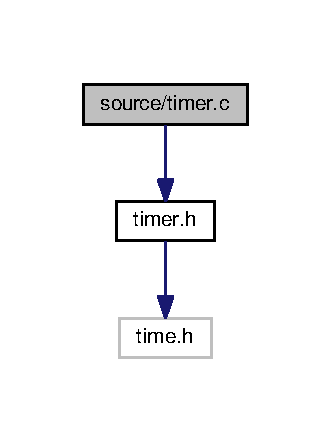
\includegraphics[width=159pt]{timer_8c__incl}
\end{center}
\end{figure}
\subsection*{Functions}
\begin{DoxyCompactItemize}
\item 
void \hyperlink{timer_8c_a7f1ca02cbf81adb4494ece96457c6c5f}{timer\+\_\+reset} ()\hypertarget{timer_8c_a7f1ca02cbf81adb4494ece96457c6c5f}{}\label{timer_8c_a7f1ca02cbf81adb4494ece96457c6c5f}

\begin{DoxyCompactList}\small\item\em Sets a new timestamp. \end{DoxyCompactList}\item 
int \hyperlink{timer_8c_aa407a36b99e4dd9072e1fb40c1d793d0}{timer\+\_\+expired} ()
\begin{DoxyCompactList}\small\item\em Checks if it has been more than T\+I\+M\+E\+\_\+\+L\+I\+M\+IT secounds since last timstamp. \end{DoxyCompactList}\end{DoxyCompactItemize}
\subsection*{Variables}
\begin{DoxyCompactItemize}
\item 
const int {\bfseries T\+I\+M\+E\+\_\+\+L\+I\+M\+IT} = 3\hypertarget{timer_8c_a23fdb30abbbaf7369615e5ea2804a8bc}{}\label{timer_8c_a23fdb30abbbaf7369615e5ea2804a8bc}

\end{DoxyCompactItemize}


\subsection{Detailed Description}
The implementation file of the timer module. 



\subsection{Function Documentation}
\index{timer.\+c@{timer.\+c}!timer\+\_\+expired@{timer\+\_\+expired}}
\index{timer\+\_\+expired@{timer\+\_\+expired}!timer.\+c@{timer.\+c}}
\subsubsection[{\texorpdfstring{timer\+\_\+expired()}{timer_expired()}}]{\setlength{\rightskip}{0pt plus 5cm}int timer\+\_\+expired (
\begin{DoxyParamCaption}
{}
\end{DoxyParamCaption}
)}\hypertarget{timer_8c_aa407a36b99e4dd9072e1fb40c1d793d0}{}\label{timer_8c_aa407a36b99e4dd9072e1fb40c1d793d0}


Checks if it has been more than T\+I\+M\+E\+\_\+\+L\+I\+M\+IT secounds since last timstamp. 

\begin{DoxyReturn}{Returns}
1 if the time limit has surpassed. 0 otherwise. 
\end{DoxyReturn}


Definition at line 19 of file timer.\+c.


\hypertarget{timer_8h}{}\section{source/timer.h File Reference}
\label{timer_8h}\index{source/timer.\+h@{source/timer.\+h}}


A library containing functions regarding the timer module.  


{\ttfamily \#include $<$time.\+h$>$}\\*
Include dependency graph for timer.\+h\+:\nopagebreak
\begin{figure}[H]
\begin{center}
\leavevmode
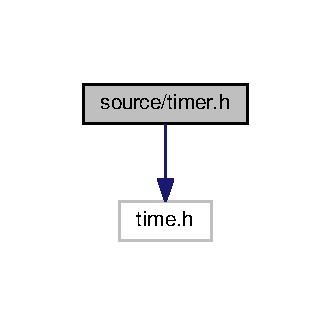
\includegraphics[width=159pt]{timer_8h__incl}
\end{center}
\end{figure}
This graph shows which files directly or indirectly include this file\+:\nopagebreak
\begin{figure}[H]
\begin{center}
\leavevmode
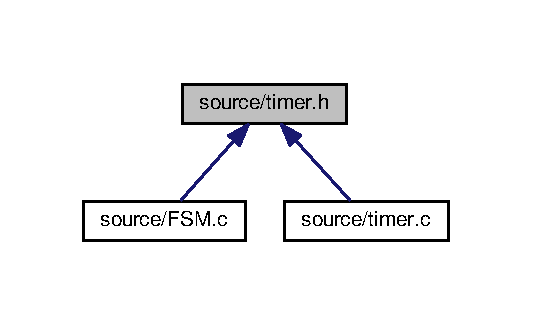
\includegraphics[width=256pt]{timer_8h__dep__incl}
\end{center}
\end{figure}
\subsection*{Functions}
\begin{DoxyCompactItemize}
\item 
void \hyperlink{timer_8h_a7f1ca02cbf81adb4494ece96457c6c5f}{timer\+\_\+reset} ()\hypertarget{timer_8h_a7f1ca02cbf81adb4494ece96457c6c5f}{}\label{timer_8h_a7f1ca02cbf81adb4494ece96457c6c5f}

\begin{DoxyCompactList}\small\item\em Sets a new timestamp. \end{DoxyCompactList}\item 
int \hyperlink{timer_8h_aa407a36b99e4dd9072e1fb40c1d793d0}{timer\+\_\+expired} ()
\begin{DoxyCompactList}\small\item\em Checks if it has been more than T\+I\+M\+E\+\_\+\+L\+I\+M\+IT secounds since last timstamp. \end{DoxyCompactList}\end{DoxyCompactItemize}


\subsection{Detailed Description}
A library containing functions regarding the timer module. 



\subsection{Function Documentation}
\index{timer.\+h@{timer.\+h}!timer\+\_\+expired@{timer\+\_\+expired}}
\index{timer\+\_\+expired@{timer\+\_\+expired}!timer.\+h@{timer.\+h}}
\subsubsection[{\texorpdfstring{timer\+\_\+expired()}{timer_expired()}}]{\setlength{\rightskip}{0pt plus 5cm}int timer\+\_\+expired (
\begin{DoxyParamCaption}
{}
\end{DoxyParamCaption}
)}\hypertarget{timer_8h_aa407a36b99e4dd9072e1fb40c1d793d0}{}\label{timer_8h_aa407a36b99e4dd9072e1fb40c1d793d0}


Checks if it has been more than T\+I\+M\+E\+\_\+\+L\+I\+M\+IT secounds since last timstamp. 

\begin{DoxyReturn}{Returns}
1 if the time limit has surpassed. 0 otherwise. 
\end{DoxyReturn}


Definition at line 27 of file timer.\+c.


%--- End generated contents ---

% Index
\backmatter
\newpage
\phantomsection
\clearemptydoublepage
\addcontentsline{toc}{chapter}{Index}
\printindex

\end{document}
